% Options for packages loaded elsewhere
\PassOptionsToPackage{unicode}{hyperref}
\PassOptionsToPackage{hyphens}{url}
%
\documentclass[
  man,floatsintext]{apa6}
\usepackage{amsmath,amssymb}
\usepackage{lmodern}
\usepackage{iftex}
\ifPDFTeX
  \usepackage[T1]{fontenc}
  \usepackage[utf8]{inputenc}
  \usepackage{textcomp} % provide euro and other symbols
\else % if luatex or xetex
  \usepackage{unicode-math}
  \defaultfontfeatures{Scale=MatchLowercase}
  \defaultfontfeatures[\rmfamily]{Ligatures=TeX,Scale=1}
\fi
% Use upquote if available, for straight quotes in verbatim environments
\IfFileExists{upquote.sty}{\usepackage{upquote}}{}
\IfFileExists{microtype.sty}{% use microtype if available
  \usepackage[]{microtype}
  \UseMicrotypeSet[protrusion]{basicmath} % disable protrusion for tt fonts
}{}
\makeatletter
\@ifundefined{KOMAClassName}{% if non-KOMA class
  \IfFileExists{parskip.sty}{%
    \usepackage{parskip}
  }{% else
    \setlength{\parindent}{0pt}
    \setlength{\parskip}{6pt plus 2pt minus 1pt}}
}{% if KOMA class
  \KOMAoptions{parskip=half}}
\makeatother
\usepackage{xcolor}
\IfFileExists{xurl.sty}{\usepackage{xurl}}{} % add URL line breaks if available
\IfFileExists{bookmark.sty}{\usepackage{bookmark}}{\usepackage{hyperref}}
\hypersetup{
  pdftitle={Measuring individual differences in the understanding of gaze cues across the lifespan},
  pdfauthor={Julia Prein1, Manuel Bohn1, Luke Maurits1, Steven Kalinke1, \& Daniel M. Haun1},
  pdflang={en-EN},
  pdfkeywords={social cognition, individual differences, gaze cues, psychometrics},
  hidelinks,
  pdfcreator={LaTeX via pandoc}}
\urlstyle{same} % disable monospaced font for URLs
\usepackage{longtable,booktabs,array}
\usepackage{calc} % for calculating minipage widths
% Correct order of tables after \paragraph or \subparagraph
\usepackage{etoolbox}
\makeatletter
\patchcmd\longtable{\par}{\if@noskipsec\mbox{}\fi\par}{}{}
\makeatother
% Allow footnotes in longtable head/foot
\IfFileExists{footnotehyper.sty}{\usepackage{footnotehyper}}{\usepackage{footnote}}
\makesavenoteenv{longtable}
\usepackage{graphicx}
\makeatletter
\def\maxwidth{\ifdim\Gin@nat@width>\linewidth\linewidth\else\Gin@nat@width\fi}
\def\maxheight{\ifdim\Gin@nat@height>\textheight\textheight\else\Gin@nat@height\fi}
\makeatother
% Scale images if necessary, so that they will not overflow the page
% margins by default, and it is still possible to overwrite the defaults
% using explicit options in \includegraphics[width, height, ...]{}
\setkeys{Gin}{width=\maxwidth,height=\maxheight,keepaspectratio}
% Set default figure placement to htbp
\makeatletter
\def\fps@figure{htbp}
\makeatother
\setlength{\emergencystretch}{3em} % prevent overfull lines
\providecommand{\tightlist}{%
  \setlength{\itemsep}{0pt}\setlength{\parskip}{0pt}}
\setcounter{secnumdepth}{-\maxdimen} % remove section numbering
% Make \paragraph and \subparagraph free-standing
\ifx\paragraph\undefined\else
  \let\oldparagraph\paragraph
  \renewcommand{\paragraph}[1]{\oldparagraph{#1}\mbox{}}
\fi
\ifx\subparagraph\undefined\else
  \let\oldsubparagraph\subparagraph
  \renewcommand{\subparagraph}[1]{\oldsubparagraph{#1}\mbox{}}
\fi
\newlength{\cslhangindent}
\setlength{\cslhangindent}{1.5em}
\newlength{\csllabelwidth}
\setlength{\csllabelwidth}{3em}
\newlength{\cslentryspacingunit} % times entry-spacing
\setlength{\cslentryspacingunit}{\parskip}
\newenvironment{CSLReferences}[2] % #1 hanging-ident, #2 entry spacing
 {% don't indent paragraphs
  \setlength{\parindent}{0pt}
  % turn on hanging indent if param 1 is 1
  \ifodd #1
  \let\oldpar\par
  \def\par{\hangindent=\cslhangindent\oldpar}
  \fi
  % set entry spacing
  \setlength{\parskip}{#2\cslentryspacingunit}
 }%
 {}
\usepackage{calc}
\newcommand{\CSLBlock}[1]{#1\hfill\break}
\newcommand{\CSLLeftMargin}[1]{\parbox[t]{\csllabelwidth}{#1}}
\newcommand{\CSLRightInline}[1]{\parbox[t]{\linewidth - \csllabelwidth}{#1}\break}
\newcommand{\CSLIndent}[1]{\hspace{\cslhangindent}#1}
\ifLuaTeX
\usepackage[bidi=basic]{babel}
\else
\usepackage[bidi=default]{babel}
\fi
\babelprovide[main,import]{english}
% get rid of language-specific shorthands (see #6817):
\let\LanguageShortHands\languageshorthands
\def\languageshorthands#1{}
% Manuscript styling
\usepackage{upgreek}
\captionsetup{font=singlespacing,justification=justified}

% Table formatting
\usepackage{longtable}
\usepackage{lscape}
% \usepackage[counterclockwise]{rotating}   % Landscape page setup for large tables
\usepackage{multirow}		% Table styling
\usepackage{tabularx}		% Control Column width
\usepackage[flushleft]{threeparttable}	% Allows for three part tables with a specified notes section
\usepackage{threeparttablex}            % Lets threeparttable work with longtable

% Create new environments so endfloat can handle them
% \newenvironment{ltable}
%   {\begin{landscape}\centering\begin{threeparttable}}
%   {\end{threeparttable}\end{landscape}}
\newenvironment{lltable}{\begin{landscape}\centering\begin{ThreePartTable}}{\end{ThreePartTable}\end{landscape}}

% Enables adjusting longtable caption width to table width
% Solution found at http://golatex.de/longtable-mit-caption-so-breit-wie-die-tabelle-t15767.html
\makeatletter
\newcommand\LastLTentrywidth{1em}
\newlength\longtablewidth
\setlength{\longtablewidth}{1in}
\newcommand{\getlongtablewidth}{\begingroup \ifcsname LT@\roman{LT@tables}\endcsname \global\longtablewidth=0pt \renewcommand{\LT@entry}[2]{\global\advance\longtablewidth by ##2\relax\gdef\LastLTentrywidth{##2}}\@nameuse{LT@\roman{LT@tables}} \fi \endgroup}

% \setlength{\parindent}{0.5in}
% \setlength{\parskip}{0pt plus 0pt minus 0pt}

% Overwrite redefinition of paragraph and subparagraph by the default LaTeX template
% See https://github.com/crsh/papaja/issues/292
\makeatletter
\renewcommand{\paragraph}{\@startsection{paragraph}{4}{\parindent}%
  {0\baselineskip \@plus 0.2ex \@minus 0.2ex}%
  {-1em}%
  {\normalfont\normalsize\bfseries\itshape\typesectitle}}

\renewcommand{\subparagraph}[1]{\@startsection{subparagraph}{5}{1em}%
  {0\baselineskip \@plus 0.2ex \@minus 0.2ex}%
  {-\z@\relax}%
  {\normalfont\normalsize\itshape\hspace{\parindent}{#1}\textit{\addperi}}{\relax}}
\makeatother

% \usepackage{etoolbox}
\makeatletter
\patchcmd{\HyOrg@maketitle}
  {\section{\normalfont\normalsize\abstractname}}
  {\section*{\normalfont\normalsize\abstractname}}
  {}{\typeout{Failed to patch abstract.}}
\patchcmd{\HyOrg@maketitle}
  {\section{\protect\normalfont{\@title}}}
  {\section*{\protect\normalfont{\@title}}}
  {}{\typeout{Failed to patch title.}}
\makeatother

\usepackage{xpatch}
\makeatletter
\xapptocmd\appendix
  {\xapptocmd\section
    {\addcontentsline{toc}{section}{\appendixname\ifoneappendix\else~\theappendix\fi\\: #1}}
    {}{\InnerPatchFailed}%
  }
{}{\PatchFailed}
\keywords{social cognition, individual differences, gaze cues, psychometrics\newline\indent Word count: X}
\usepackage{lineno}

\linenumbers
\usepackage{csquotes}
\usepackage{setspace}
\captionsetup[figure]{font={stretch=1}}
\ifLuaTeX
  \usepackage{selnolig}  % disable illegal ligatures
\fi

\title{Measuring individual differences in the understanding of gaze cues across the lifespan}
\author{Julia Prein\textsuperscript{1}, Manuel Bohn\textsuperscript{1}, Luke Maurits\textsuperscript{1}, Steven Kalinke\textsuperscript{1}, \& Daniel M. Haun\textsuperscript{1}}
\date{}


\shorttitle{Gaze cue understanding}

\authornote{

Correspondence concerning this article should be addressed to Julia Prein, Max Planck Institute for Evolutionary Anthropology, Deutscher Platz 6, 04103 Leipzig, Germany. E-mail: \href{mailto:julia_prein@eva.mpg.de}{\nolinkurl{julia\_prein@eva.mpg.de}}

}

\affiliation{\vspace{0.5cm}\textsuperscript{1} Department of Comparative Cultural Psychology, Max Planck Institute for Evolutionary Anthropology, Leipzig, Germany}

\abstract{%
To explain and predict the behavior of agents, we use social cognition: we represent and reason about others' perspectives, knowledge, intentions, beliefs, and preferences. However, traditional measures of social cognition (e.g., false belief change-of-location tasks) often lack satisfactory psychometric properties: they are not designed to capture variation \emph{between} children and rely on low trial numbers, dichotomous measures, and group averages. This has profound implications for what these studies can show. Poor measurement of social cognition on an individual level may conceal relations between different aspects of cognition and may obscure developmental change. To fully understand how social-cognitive abilities emerge and relate to each other, we need new tools that can reliably measure individual differences.
We designed a balloon-finding task to study social cognition in young children and adults to approach this issue. We concentrate on an essential ability that is involved in many social-cognitive reasoning processes: gaze cue understanding -- the ability to locate and use the attentional focus of an agent. Our interactive task works across devices and enables supervised and unsupervised, as well as in-person and remote testing. The implemented spatial layout allows for discrete and continuous measures of participants' click imprecision and is easily adaptable to different study requirements.
Here we show that our task induces inter-individual differences in a child (N = XXX) and an adult (N = XXX) sample. Our two study versions and data collection modes yield comparable results that show substantial developmental gains: the older children are, the more accurately they locate the target. High internal consistency and test-retest reliability estimates underline that the captured variation is systematic. Furthermore, we find first evidence for the external validity of our task: the measured performance in gaze cue understanding relates to children's real-life social surroundings. This work shows a promising way forward in the study of individual differences in social cognition and will help us explore the in(ter)dependence of our core social-cognitive processes in greater detail.
}



\begin{document}
\maketitle

\hypertarget{introduction}{%
\section{Introduction}\label{introduction}}

Social cognition - representing and reasoning about an agent's perspectives, knowledge states, intentions, beliefs, and preferences to explain and predict their behavior - is among the most-studied phenomena in developmental research.
In recent decades, much progress has been made in determining the average age at which a specific social-cognitive ability emerges in development (Gopnik \& Slaughter, 1991; Candida C. Peterson, Wellman, \& Slaughter, 2012; Rakoczy, 2022; \textbf{wellman2001metaanalysisa?}; \textbf{wellman2004scalinga?}).

One of the most commonly applied prototypical measures for social cognition is the Sally-Anne task (Baron-Cohen, Leslie, \& Frith, 1985).
Here, children watch a short sequence of events (often acted out or narrated by the experimenters).
A doll called Sally puts her marble into a basket.
After Sally leaves the scene, a second doll named Anne takes the marble and moves it into a box.
Participants then get asked where Sally will look for her marble once she returns.
The outcome measures false belief understanding in a dichotomous way:
children pass the task if they take the protagonist's epistemic state into account and answer that she will look into the basket.
Many years of research utilizing these verbal change-of-location tasks suggest that children develop belief-representing abilities at four to five years of age (for a review, see \textbf{wellman2001metaanalysisa?}).
Several cross-cultural studies supported this evidence (Barrett et al., 2013; Callaghan et al., 2005; cf. Mayer \& Träuble, 2015).
However, from this age onwards, the change-of-location task shows ceiling effects and has very limited diagnostic value (V. S. \&. B. Repacholi, 2003).
As Wellman (2012) put it, ``it's really only passing/failing one sort of understanding averaged across age'' (p.~317).
Therefore, the focus has been to track change at an (age-) group level within a narrow developmental time frame and with a strong emphasis on a single social-cognitive ability.

Although humans substantially differ in their behavior, thoughts, and motivations, researchers often regard variability as cumbersome or reinterpret it as error variance, therefore neglecting and trivializing individual differences (Kidd, Donnelly, \& Christiansen, 2018).
Consequently, little consensus has been reached on the interrelation or independence of social-cognitive abilities (termed `structure of social cognition' by Happé, Cook, \& Bird, 2017).

However, identifying variability in social-cognitive abilities and factors influencing those could be vital in theory building (e.g., to test causal predictions) and design interventions (Happé et al., 2017).
For example, the structure of variability could be used to provide evidence for two accounts: (1) \emph{developmental lags} (i.e., whether children differ in their speed of acquiring new conceptual insights into the understanding of the mind), and (2) \emph{genuine variation} (i.e., whether children differ in their ease or fluency in (applying) these social-cognitive abilities) (Hughes \& Devine, 2015). Stenhaug, Ram, and Frank (2021) have argued for the differentiation between stage models (i.e., synchronization in developmental changes across distinct domains) and modular theories (i.e., particular aspects of development proceed on their own schedule).
In addition, individual difference studies are useful for identifying antecedent factors as potential developmental causes, consequences of an early or late social-cognitive development, and qualitative differences in the actual social life (Bartsch \& Estes, 1996; Keenan, 2003).
Therefore, we argue that studying the co-development of social-cognitive abilities, variation in the individual's pace of mastering developmental milestones, and which factors influence a child's proficiency requires us to take individual differences seriously -- both theoretically and methodologically.

Some studies have already examined individual differences in social cognition (for an overview, see Hughes \& Devine, 2015; Slaughter, 2015).
These individual differences studies usually focus on three different kinds of relationships between social-cognitive abilities and:
(1) family influences, (2) other cognitive constructs, and (3) social outcome measures (for an overview, see V. S. \&. B. Repacholi, 2003).

The first subgroup covers studies on social-cognitive abilities and parenting practices (for a review, see Pavarini, de Hollanda Souza, \& Hawk, 2013), attachment quality (e.g., Astor et al., 2020), mental state talk (Gola, 2012; Hughes, Ensor, \& Marks, 2011; Lecce, Bianco, Devine, Hughes, \& Banerjee, 2014), and family background (education, occupation, sibling interaction, childcare) {[}Dunn, Brown, Slomkowski, Tesla, and Youngblade (1991); Cutting and Dunn (1999); bulgarelli2016social{]}.
In the second subgroup, individual differences studies include the interplay of social and physical cognition (Herrmann, Hernández-Lloreda, Call, Hare, \& Tomasello, 2010), executive functions (Benson, Sabbagh, Carlson, \& Zelazo, 2012; Buttelmann, Kühn, \& Zmyj, 2021; Stephanie M. Carlson \& Moses, 2001; Stephanie M. Carlson, Moses, \& Claxton, 2004; Hughes \& Ensor, 2007), and language abilities (McEwen et al., 2007 Mar-Apr; Milligan, Astington, \& Dack, 2007; Okumura, Kanakogi, Kobayashi, \& Itakura, 2017).
The third subgroup encompasses studies on social cognition and prosociality (for a review, see Imuta, Henry, Slaughter, Selcuk, \& Ruffman, 2016; Walker, 2005),
stereotypes and resource allocations (Rizzo \& Killen, 2018), and moral intentions (Sodian et al., 2016).

Correlational approaches have also been used to argue for and test assumptions of cognitive development theories (Kidd et al., 2018; Mundy et al., 2007; Underwood, 1975).

Frequently, developmental psychologists are surprised to find minor or no association between constructs that are thought to be theoretically related (e.g., Sodian et al., 2016).
This might be because traditional measures of social cognition are not designed to capture variation between children:
they often rely on low trial numbers, small sample sizes, and dichotomous measures.
Hedge, Powell, and Sumner (2018) argued that cognitive tasks often become well-established by displaying robust effects across studies.
The authors could show that this usually does not emerge due to high measurement variance but relatively low between-subject variability, concluding that popular cognitive tasks may reliably measure group differences but not individual differences (termed ``reliability paradox'').
Similarly, Pronk, Molenaar, Wiers, and Murre (2021) reasoned that accurate reliability estimates are needed to judge how well a particular cognitive test is suited to draw inferences about individuals.
A recent review underlined reoccurring issues in standardization, validity, reliability, and sensitivity to developmental change: alarmingly few theory of mind measures reported empirically validated psychometric properties (Beaudoin, Leblanc, Gagner, \& Beauchamp, 2020) or showed poor test-retest reliability (Mayes, Klin, Tercyak, Cicchetti, \& Cohen, 1996) (but cf Hughes et al., 2000).

Even studies focusing on individual differences often use behavioral forced-choice paradigms {[}e.g., carlson2004individual; Walker (2005){]}.
Few studies that do realize continuous measures often administer (theory of mind) scales and conventionally compute aggregate scores (across tasks or trials), therefore neglecting the issue of measurement error (Hughes et al., 2011).
This way, a particular social-cognitive ability in question is still assessed categorically on a trial basis (e.g., Bulgarelli \& Molina, 2016; Buttelmann et al., 2021; Rizzo \& Killen, 2018). In addition, individual differences are only identified in the age of onset of the social-cognitive ability and not in performance or competence (V. S. \&. B. Repacholi, 2003).
This has profound implications for what these studies can show.
Poor measurement of social cognition on an individual level may conceal relations between different aspects of cognition and may obscure developmental change.

Therefore, developmental psychology faces a dilemma: many research questions are questions about individual differences, yet, there is a lack of tasks to measure these individual differences reliably.
To capture the emergence of social-cognitive abilities and related social factors in greater precision and detail, we must consequently address the methodological limitations of existing study designs (Hughes et al., 2011; Hughes \& Leekam, 2004).

Schaafsma, Pfaff, Spunt, and Adolphs (2015) compiled a ``wish-list'' for new social-cognitive paradigms. They advocated for parametric measures covering proficiency as a range, avoiding floor and ceiling effects, and showing satisfactory test-retest reliability estimates.
In valid and reliable tasks, differences in test scores should correspond to differences in the social-cognitive ability and systematically order individuals in the same way.
Additionally, tasks should allow for use within an fMRI scanner.
With an easily administrable test procedure, larger sample sizes can be collected to estimate the potentially small effect of inter-individual differences.

Additionally, it has been argued that social-cognitive abilities should not be treated as an all-or-nothing matter (e.g., dichotomously in pass/fail situations) but as abilities on a continuum (Beaudoin et al., 2020; Hughes \& Devine, 2015; Keenan, 2003).
Task batteries might be better suited to cover a range of social-cognitive abilities V. S. \&. B. Repacholi (2003).
Schaafsma et al. (2015) proposed that first basic social-cognitive processes should be relatively well understood before advancing to more complex social-cognitive abilities.

Another goal in creating new tasks should be to focus on the face value:
we want to measure the underlying social-cognitive ability as straight-forward and directly as possible.
The task should serve as a proxy for behavior as it appears in the real world (B. Repacholi \& Slaughter, 2004; V. S. \&. B. Repacholi, 2003).
Importantly, we can assess whether the task shows external validity by evaluating the relationship with related constructs and factors of children's social surroundings.

Therefore, we aim to make individual differences measurable in a systematic and reliable way.
We want to create a task that induces variation between children to get precise person-specific estimates.
To approach this issue, we focus on a continuous measure and short trials that facilitate more than a dozen replicates per subject.
A standardized, easily accessible test procedure helps us to enable data collection at scale.
Since data collection with families requires much organizational effort, we want to enable data collection in-person with supervision as well as remotely without supervision.

In our first novel task, we concentrate on the fundamental ability that is involved in many social-cognitive reasoning processes:
gaze cue understanding - the ability to locate and use the attentional focus of an agent.
The first component of this ability is often termed gaze following - turning one's eyes in the same direction as the gaze of another agent - and has been studied intensively (Astor, Thiele, \& Gredebäck, 2021; Byers-Heinlein et al., 2021; Coelho, George, Conty, Hugueville, \& Tijus, 2006; Del Bianco, Falck-Ytter, Thorup, \& Gredebäck, 2019; Frischen, Bayliss, \& Tipper, 2007; Hernik \& Broesch, 2019; Itakura \& Tanaka, 1998; Lee, Eskritt, Symons, \& Muir, 1998; Moore, 2008; Shepherd, 2010; Tomasello, Hare, Lehmann, \& Call, 2007).
Following an agent's gaze provides insights into their intentions, thoughts, and feelings by acting as a `front end ability' (Brooks \& Meltzoff, 2005, p. 535).
In our definition, gaze cue understanding goes one step further by including the \emph{acting on the gaze-cued location} - therefore, using the available social information to guide one's behavior as needed in real-life conditions.

\hypertarget{task-design}{%
\section{Task design}\label{task-design}}

\hypertarget{implementation}{%
\subsection{Implementation}\label{implementation}}

Our balloon finding task is presented as an interactive web app. The task is portable across devices and web browsers and does not require any installation. An advantage of online testing is that our testing procedure is standardized across participants. By using pre-recorded study instructions, no interaction with the experimenter is necessary during the study. The code is open-source (\url{https://github.com/ccp-eva/gafo-demo}) and a live demo version can be found under: \url{https://ccp-odc.eva.mpg.de/gafo-demo/}.

The web app was programmed in \texttt{JavaScript}, \texttt{HTML5}, \texttt{CSS} and \texttt{PHP}. For stimulus presentation, a scalable vector graphic (SVG) composition was parsed. This way, the composition scales according to the user's view port without loss of quality, while keeping the aspect ratio and relative object positions constant. Furthermore, SVGs allow us to define all composite parts of the scene (e.g., pupil of the agent) individually. This is needed for precisely calculating exact pupil and target locations and sizes. Additionally, it makes it easy to adjust the stimuli and, for example, add another agent to the scene. The web app generates two file types: (1) a text file (.json) containing meta-data, trial specifications and participants' click responses, and (2) a video file (.webm) of the participant's webcam recording. These files can either be sent to a server or downloaded to the local device.

\hypertarget{stimuli}{%
\subsection{Stimuli}\label{stimuli}}

Our newly implemented task features an online game where children or adults are asked to search for a balloon. The events proceed as follows (see Figure \ref{fig:fig1}B and C). An animated agent (a sheep, monkey, or pig) looks out of a window of a house. A balloon (i.e., target; blue, green, yellow, or red) is located in front of them. The target then falls to the ground. At all times, the agent's gaze tracks the movement of the target. That is, the pupils and iris of the agent move in a way that their center aligns with the center of the target. While the distance of the target's flight depends on the final location, the target moves at a constant speed. Participants are then asked to locate the target: they respond by touching or clicking on the screen. Visual access to the target's true location is manipulated by a hedge. Participants either have full, partial, or no visual access to the true target location. When partial or no information about the target location is accessible, participants are expected to use the agent's gaze as a cue.

To keep participants engaged and interested, the presentation of events is accompanied by cartoon-like effects. Each trial starts with an attention-getter: an eye-blinking sound plays while the pupils and iris of the agent enlarge (increase to 130\%) and change in opacity (decrease to 75\%) for 0.3 sec.~The landing of the target is accompanied by a tapping sound. Once the target landed, the instructor's voice asks ``Where is the balloon?''. For confirming the participant's click, a short plop sound plays and a small orange circle appears at the location of choice. If no response is registered within 5 secs after the target landed, an audio prompt reminds the participant to respond.

\hypertarget{trials}{%
\subsection{Trials}\label{trials}}

Trials differ in the amount of visual access that participants have to the final target position. Before the test trials start, participants complete four training trials during which they familiarize themselves with clicking the screen. In the first training trial, participants have full visual access to the target flight and the target's end location and are simply asked to click on the visible balloon. In the second and third training trials, participants have partial access: they witness the target flight but cannot see the target's end location. They are then asked to click on the hidden balloon, i.e., the location where they saw the target land. In test trials, participants have no visual access to the target flight or the end location. Participants are expected to use the agent's gaze as a cue to locate the target. The first trial of each type comprises a voice-over description of the presented events. The audio descriptions explicitly state that the agent is always looking at the target (see Appendix for audio script). After the four training trials, participants receive 15 test trials. The complete sequence of four training trials and 15 test trials can be easily completed within 5-10 minutes.

\hypertarget{study-versions}{%
\subsection{Study versions}\label{study-versions}}

We designed two study versions which differ in the final hiding place of the target and, consequently, on the outcome measure: a \emph{hedge version} (continuous) and a \emph{box version} (discrete). Both versions use the same first training trial and then differ in the consecutive training and test trials.
In the hedge version, participants have to indicate their estimated target location directly on a hedge. Here, the dependent variable is imprecision, which is defined as the absolute difference between the target center and the x coordinate of the participant's click.
In the box version, the target lands in a box and participants are asked to click on the box that hides the target. Researchers have the choice how many boxes are shown: one up to eight boxes can be displayed as potential hiding locations. Here, we use a categorical outcome (i.e., which box was clicked) to calculate the proportion of correct responses.
Note that in the test trials of both versions, the target flight is covered by a hedge. In the hedge version, the hedge then shrinks to a minimum height required to cover the target's end location. In the box version, the hedge shrinks completely. The boxes then hide the target's final destination (see Figure \ref{fig:fig1}B and C).






\begin{figure}

{\centering 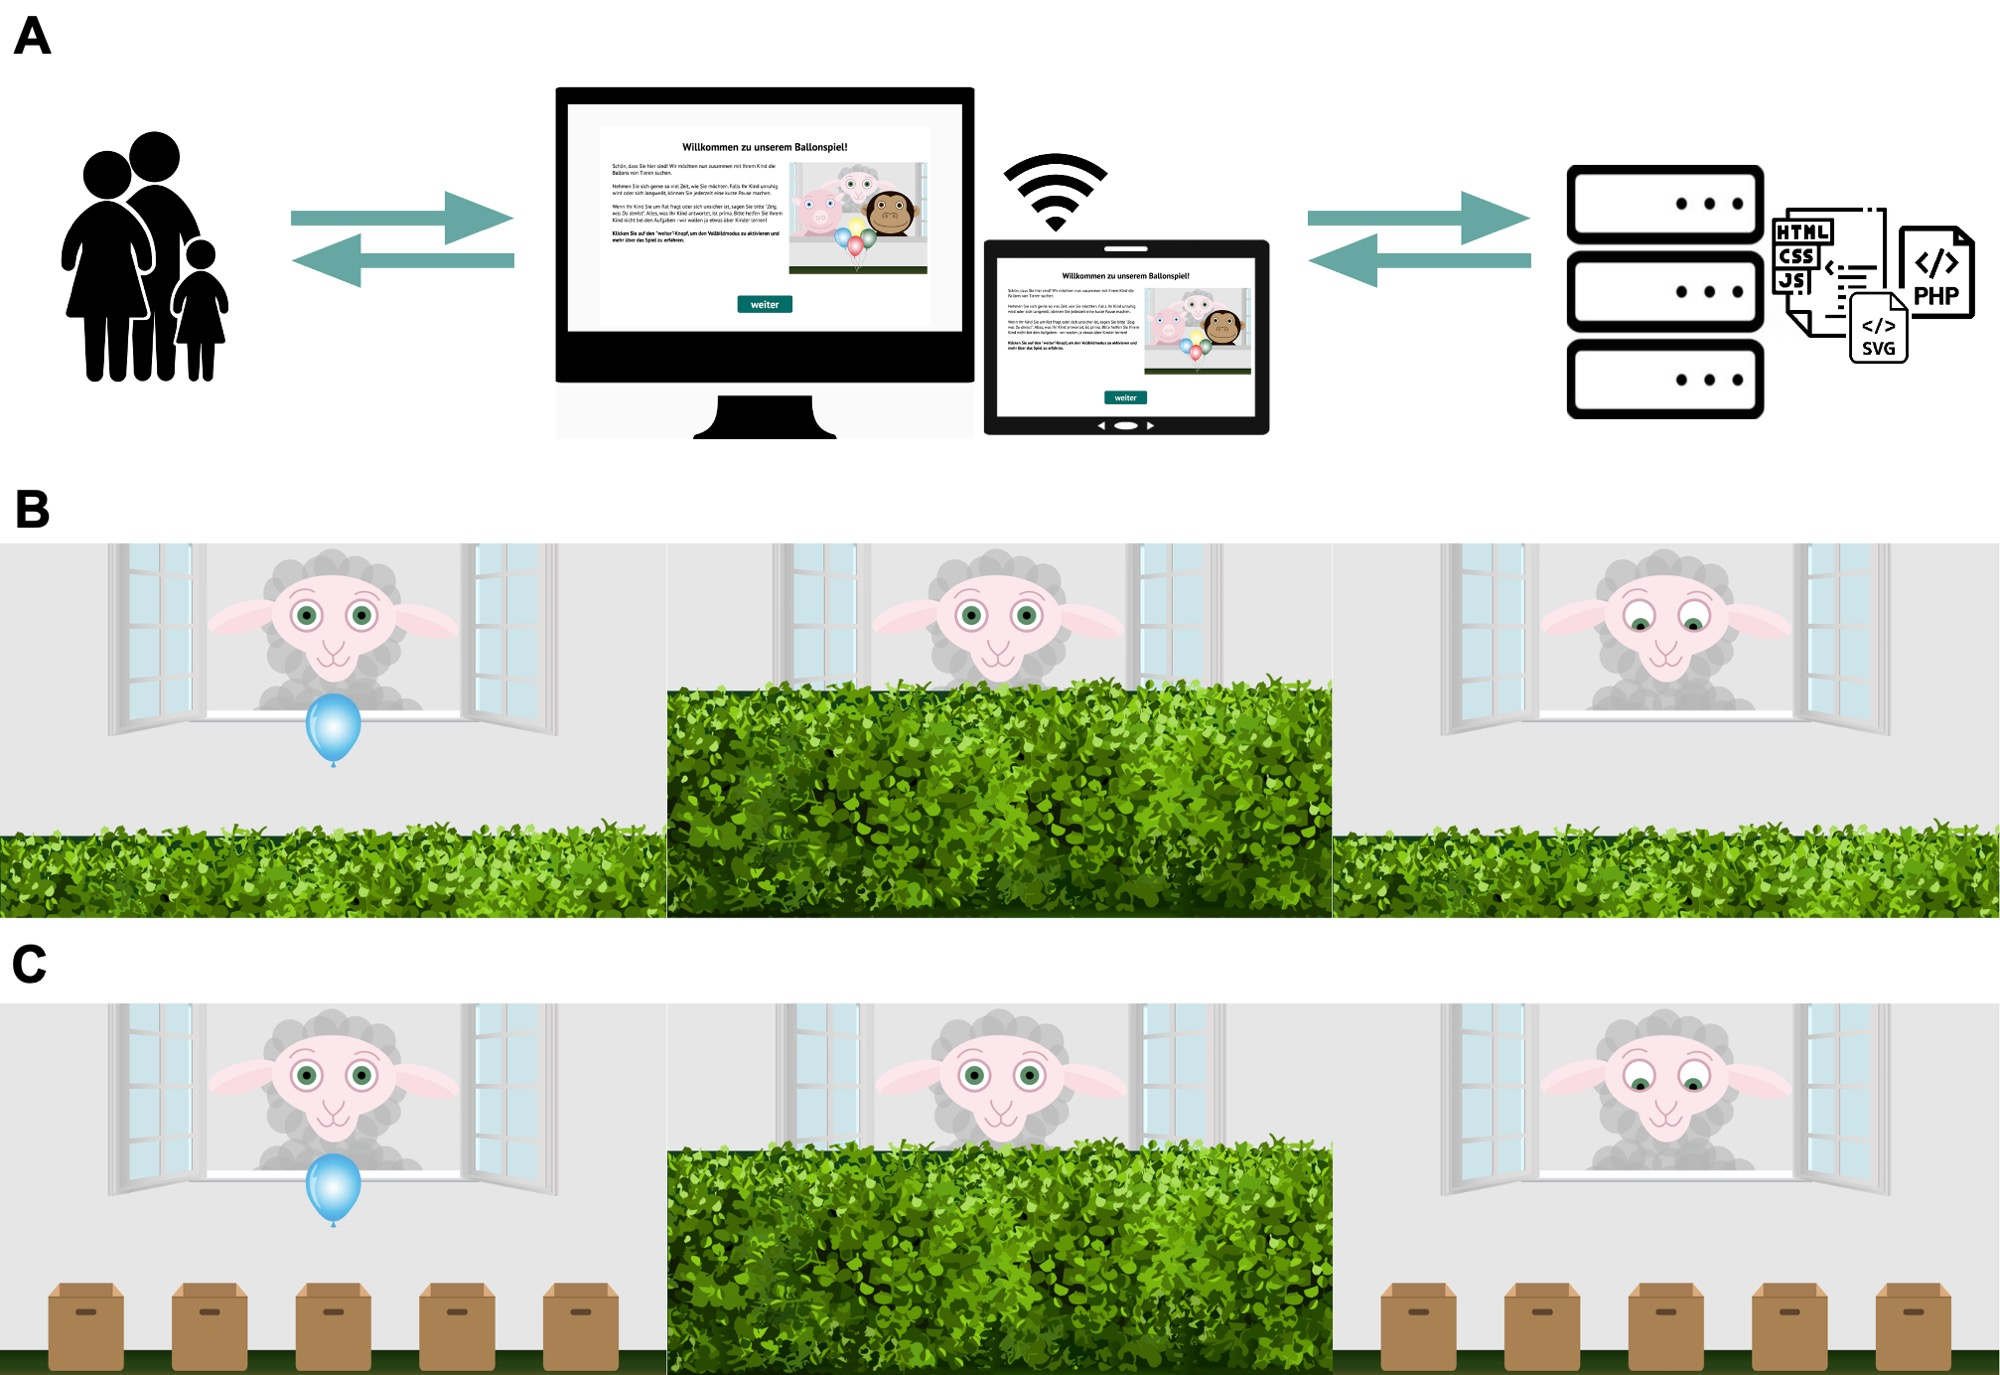
\includegraphics[width=1\linewidth]{../figures/gafo_procedure} 

}

\caption{\textbf{Study setup}.
(A) Infrastructure for online testing. (i) Subjects aged 3 -- 99+ can participate. Data collection can take place anywhere: online, in kindergartens or research labs. (ii) The task is presented as a website that works across devices. (iii) The scripts for the website and the recorded data are stored on secure local servers.
(B) Hedge version (continuous) of the balloon finding task. (i) The agent stands in a window with the target in front of them. (ii) A hedge grows and covers the target. (iii) The target falls to a random location on the ground. The agent's eyes track the movement of the target.
(C) Box version (discrete) of the balloon finding task. Number of boxes (min. 1; max. 8) as potential hiding locations can be set according to the researcher's need.}\label{fig:fig1}
\end{figure}

\hypertarget{randomization}{%
\subsection{Randomization}\label{randomization}}

All agents and target colors appear equally often and are not repeated in more than two consecutive trials. The randomization of the target end location depends on the study version. In the hedge version, the full width of the screen is divided into ten bins. Exact coordinates within each bin are then randomly generated. In the box version, the target randomly lands in one of the boxes. As with agent and color choice, each bin/box occurs equally often and can only occur twice in a row.

\hypertarget{individual-differences}{%
\section{Individual differences}\label{individual-differences}}

Our first aim was to assess whether our balloon finding task induces inter-individual variation in a child and adult sample. Furthermore, we were interested in how the data collection mode influences responses.

Methods, sample size and analysis were pre-registered: \url{https://osf.io/snju6} (child sample) and \url{https://osf.io/r3bhn} (adult sample). Participants were equally distributed across the two study versions. The study was approved by an internal ethics committee at the Max Planck Institute for Evolutionary Anthropology. Data was collected between May and October 2021.

\hypertarget{participants}{%
\subsection{Participants}\label{participants}}

We collected data from an in-person child sample, a remote child sample, and a remote adult sample.
In-person testing with children took place in kindergartens in Leipzig, Germany. The in-person child sample consisted of
120 children, including
40 3-year-olds
(mean = 41.45 months,
SD = 3.85,
range = 36
- 47,
22 girls),
40 4-year-olds
(mean = 54.60 months,
SD = 3.10,
range = 48
- 59,
19 girls),
and 40 5-year-olds
(mean = 66.95 months,
SD = 3.39,
range = 60
- 71,
22 girls).

For our remote child sample, we recruited families via an internal database. The remote child sample included 147 children, including
45 3-year-olds
(mean = 42.62 months,
SD = 3.35,
range = 36
- 47,
14 girls),
47 4-year-olds
(mean = 52.64 months,
SD = 3.40,
range = 48
- 59,
25 girls),
and 55 5-year-olds
(mean = 65.11 months,
SD = 3.77,
range = 60
- 71,
27 girls). Children in our sample grow up in an industrialized, urban Central-European context. Information on socioeconomic status was not formally recorded, although the majority of families come from mixed, mainly mid to high socioeconomic backgrounds with high levels of parental education.

Adults were recruited via \emph{Prolific} (Palan \& Schitter, 2018). \emph{Prolific} is an online participant recruitment service from the University of Oxford with a predominantly European and US-american subject pool. Participants consisted of 50 and 50 English-speakers with an average age of 31.92 and 30.76 years (SD = 12.15 and 9.12, range = 18 and 19 - 63 and 59, 36 and 28 females).
For completing the study, subjects were payed above the fixed minimum wage (in average £10.00 per hour).

\hypertarget{procedure}{%
\subsection{Procedure}\label{procedure}}

Children in our in-person sample were tested on a tablet in a quiet room in their kindergarten. An experimenter guided the child through the study. Children in the remote sample received a personalized link to the study website and families could participate at any time or location they wanted. In the beginning of the online study, families were invited to enter our ``virtual institute'' and were welcomed by an introductory video of the study leader, shortly describing the research background and further procedure. Then, caregivers were informed about data security and were asked for their informed consent. They were asked to enable the sound and seat their child centrally in front of their device. Before the study started, families were instructed how to setup their webcam and enable the recording permissions. We stressed that caregivers should not help their children. Study participation was video recorded whenever possible in order to ensure that the answers were generated by the children themselves.
Depending on the participant's device, the website automatically presented the hedge or box version of the study. For families that used a tablet with touchscreen, the hedge version was shown. Here, children could directly click on the touchscreen themselves to indicate where the target is. For families that used a computer without touchscreen, the website presented the box version of the task. We assumed that younger children in our sample would not be acquainted with the usage of a computer mouse. Therefore, we asked children to point to the screen, while caregivers were asked to act as the ``digital finger'' of their children and click on the indicated box.

All participants received 15 test trials. In the box version, we decided to adjust the task difficulty according to the sample: children were presented with five boxes while adults were presented with eight boxes as possible target locations.

\hypertarget{analysis}{%
\subsection{Analysis}\label{analysis}}

All test trials without voice over description were included in our analyses. We ran all analyses in R version 4.2.0 (2022-04-22) (R Core Team, 2022). Regression models were fit as Bayesian generalized linear mixed models (GLMMs) with default priors for all analyses, using the function \texttt{brm} from the package \texttt{brms} (Bürkner, 2017, 2018).

To estimate the developmental trajectory of gaze cue understanding and the effect of data collection mode, we fit a GLMM predicting the task performance by age (in months, z-transformed) and data collection mode (reference category: in-person supervised). The model included random intercepts for each participant and each target position, and a random slope for symmetric target position within participants (model notation in \texttt{R:\ performance\ \textasciitilde{}\ age\ +\ datacollection\ +\ (symmetricPosition\ \textbar{}\ subjID)\ +\ (1\ \textbar{}\ targetPosition)}). Here, \texttt{targetPosition} refers to the exact bin/box of the target, while \texttt{symmetricPosition} refers to the absolute distance from the stimulus center (i.e., smaller value meaning more central target position). We expected that trials could differ in their difficulty depending on the target centrality and that these these item effects could vary between participants.

For the hedge version, performance was defined as the absolute click distance between the target center and the click X coordinate, scaled according to target widths, and modeled by a \texttt{lognormal} distribution. For the box version, the model predicted correct responses (0/1) using a \texttt{Bernoulli} distribution with a logit link function. We inspected the posterior distribution (mean and 95\% Confidence Interval (CI)) for the age and data collection estimates.

\hypertarget{results}{%
\subsection{Results}\label{results}}










\begin{figure}

{\centering 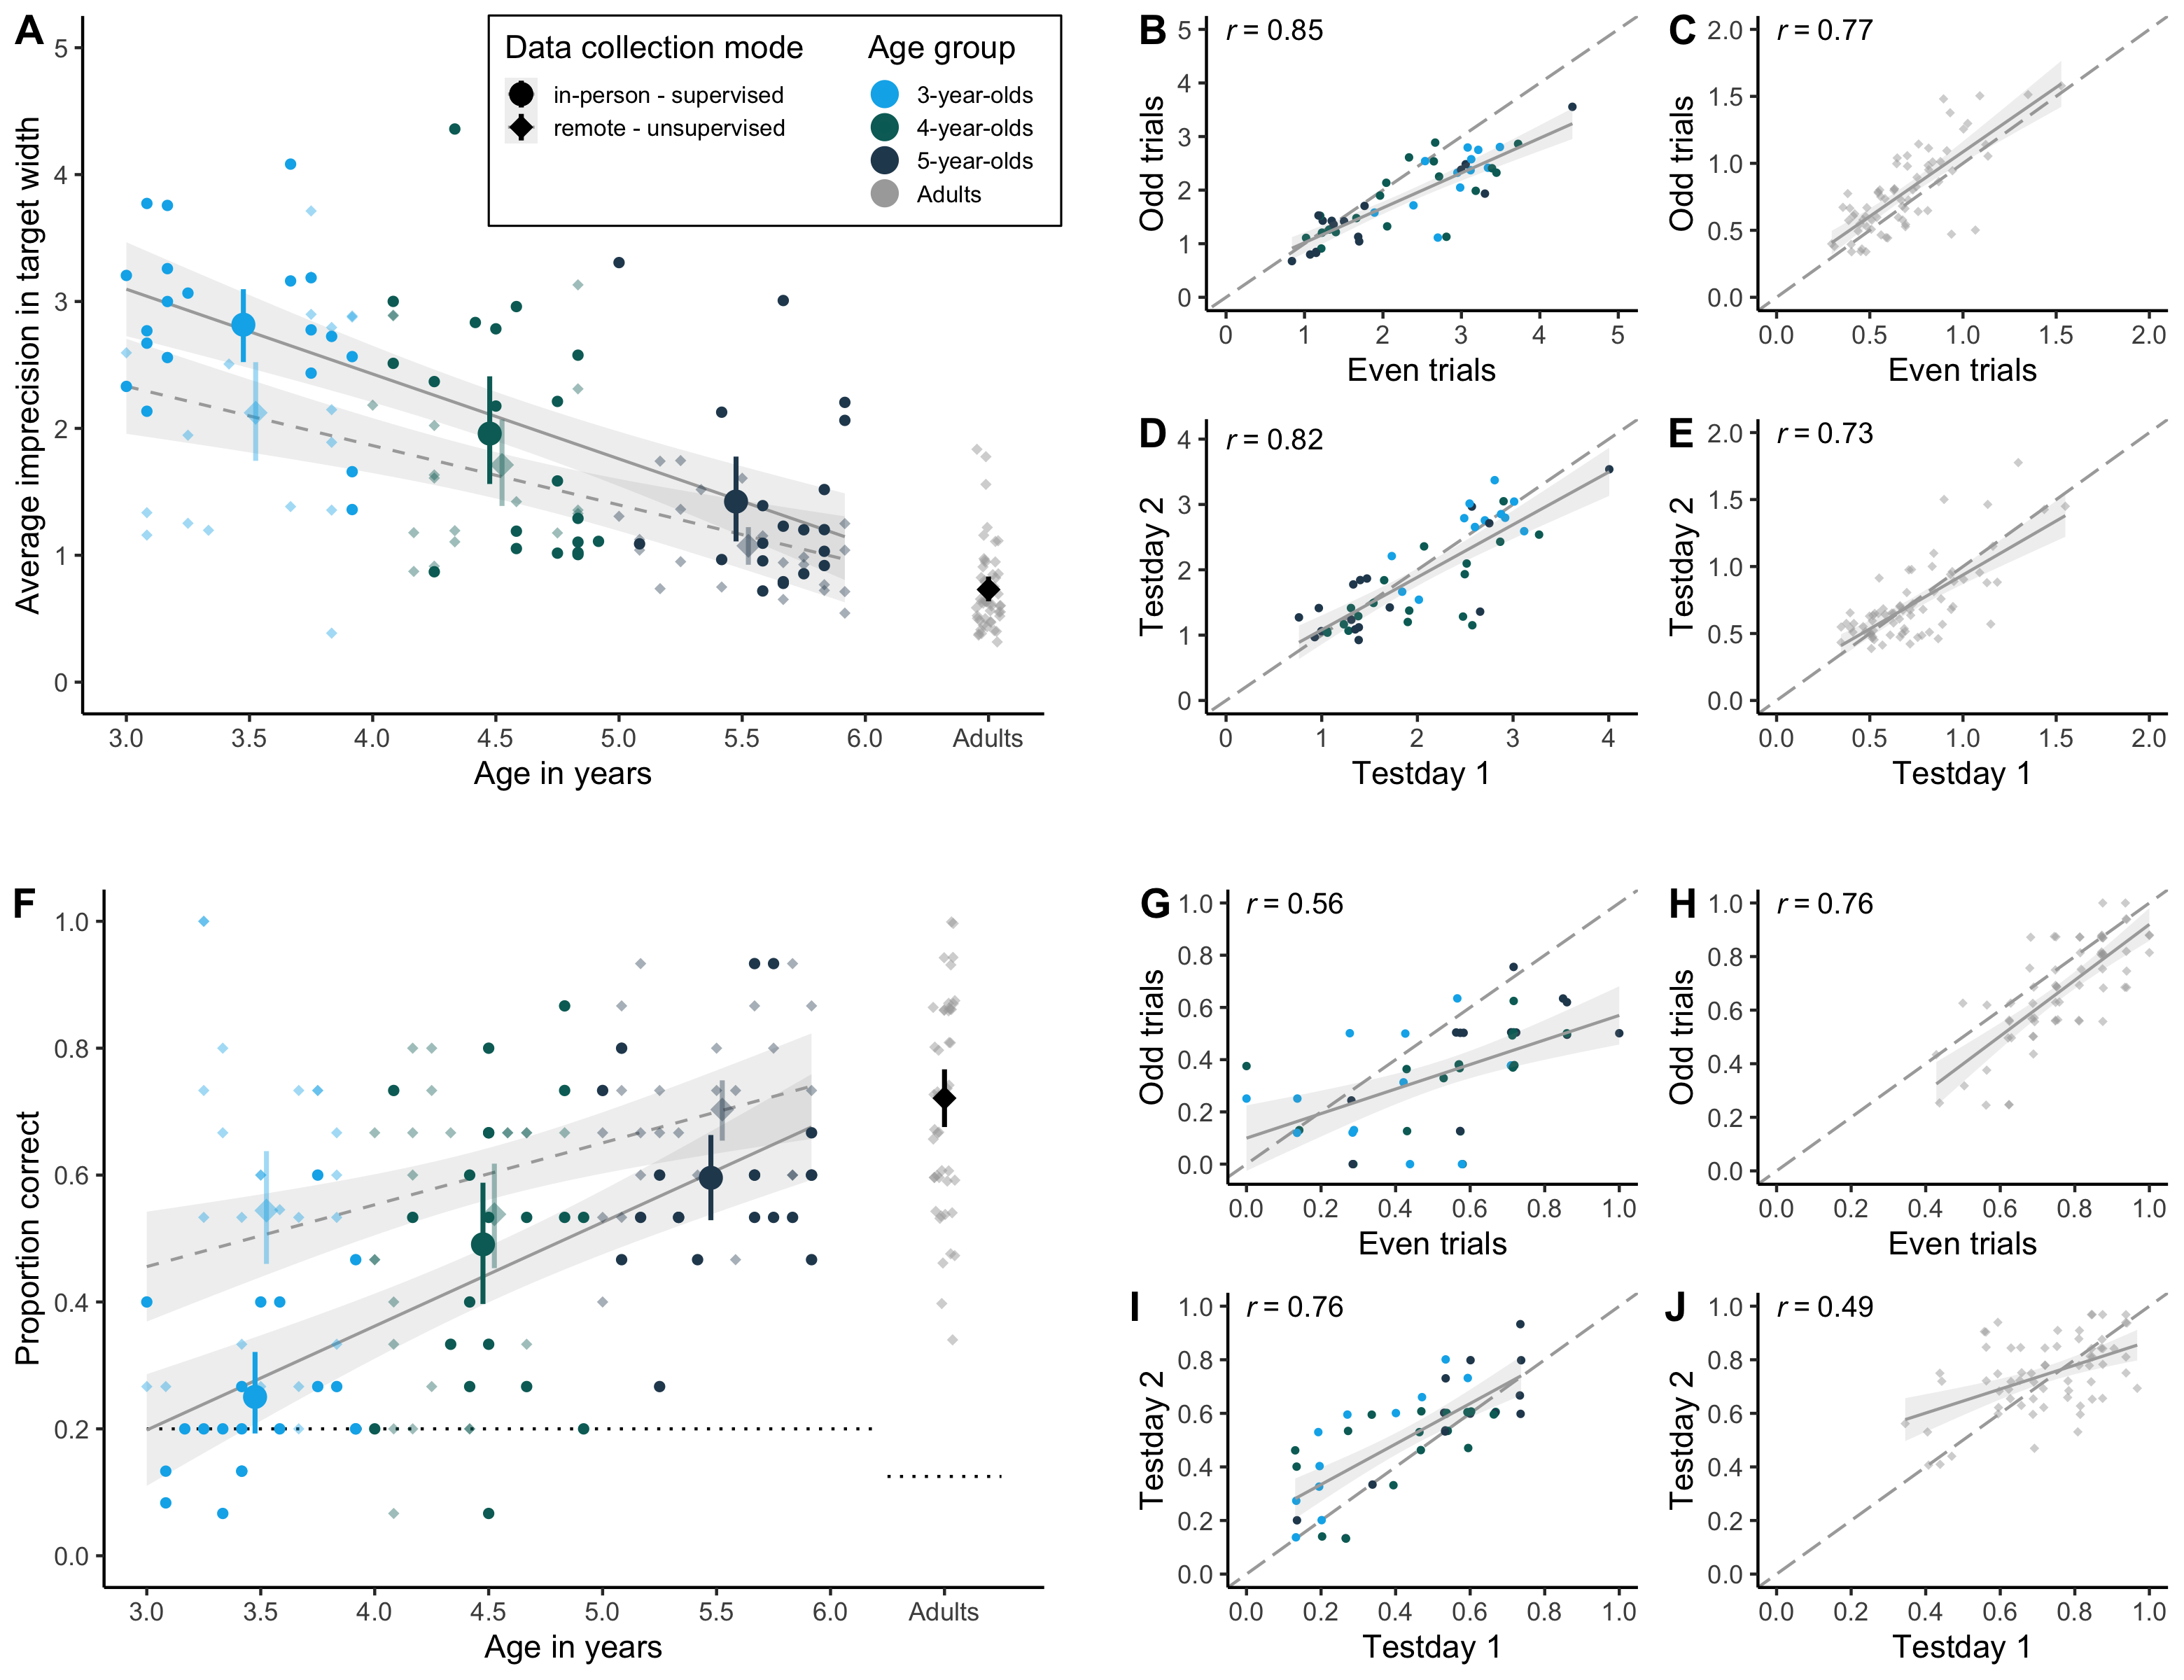
\includegraphics[width=1\linewidth]{../figures/gafo_results} 

}

\caption{\textbf{Measuring inter-individual variation}.
(A) Developmental trajectory in continuous hedge version. Performance is measured as average imprecision, i.e., the absolute distance between the target's center and the participant's click. The unit of imprecision is counted in the width of the target, i.e., a participant with an imprecision of 1 clicked in average one target width to the left or right of the true target center.
(B) Internal consistency (odd-even split) in hedge child sample. (C) Internal consistency in hedge adult sample. (D) Test-retest reliability in hedge child sample. (E) Test-retest reliability in hedge adult sample.
(F) Developmental trajectory in discrete box version. Performance is measured as the proportion of correct responses, i.e., how many times the participant clicked on the box that actually contained the target. Dotted black line shows level of performance expected by chance (for child sample 20\%, i.e., 1 out of 5 boxes; for adult sample 12.5\%, i.e., 1 out of 8 boxes).
(G) Internal consistency (odd-even split) in box child sample. (H) Internal consistency in box adult sample. (I) Test-retest reliability in box child sample. (J) Test-retest reliability in box adult sample.
Regression lines with 95\% CI show smooth conditional mean based on a linear model (generalized linear model for box version), with \emph{Pearson}'s correlation coefficient \emph{r}.
Large points with 95\% CI (based on non-parametric bootstrap) represent performance means by age group (binned by year).
Small points show the mean performance for each subject. Shape of data points represents data collection mode: opaque circles for in-person supervised data collection, translucent diamonds for remote unsupervised data collection. Color of data points denotes age group.}\label{fig:fig2}
\end{figure}

We found a strong developmental effect: with increasing age, participants got more and more accurate in locating the target. In the hedge version, children's click imprecision decreased with age, while, in the box version the proportion of correct responses increased (see Figure \ref{fig:fig2}A and F). Most participants in the box version performed above chance level. By the end of their sixth year of life, children came close to the adult's proficiency level. Most importantly, however, we found substantial inter-individual variation across study versions and age groups. For example, some three-year-olds were more precise in their responses than some five-year-olds. Even though variation is smaller, we even find inter-individual differences in the adult sample.

As Figure \ref{fig:fig2}A and F show, our remotely collected child data resembled the data from the kindergarten sample.
We found evidence that responses of children participating remotely were slightly more precise. This difference was mainly driven by the younger participants and especially prominent in the box version of the task. It is conceivable that caregivers were especially prone to influence the behavior of younger children. In the box version, caregivers might have had more opportunities to interfere since they carried out the clicking for their children.\footnote{In an exploratory analysis, we coded parental behavior and environmental factors during remote unsupervised testing. We focused on the subsample with the greatest performance difference between data collection modes: the three-year-olds in the box version of the task (n = 16). We reasoned that if parental interference cannot explain the greatest performance difference in our sample, the effects would be negligible in the remaining sample. Based on our model comparison, we conclude that there is no clear evidence of a stable effect of parental interference. See Supplements for further detail.}

Our GLMM analysis corroborated the visual inspection of the data: in the hedge version, the estimates for age (\(\beta\) = -0.32; 95\% CI {[}-0.41; -0.24{]}) and data collection mode -0.32 (95\% CI {[}-0.49; -0.14{]}) were negative and reliably different from zero.
In the box version, the estimate of age (\(\beta\) =0.63 (95\% CI {[}0.40; 0.88{]}) and the estimate of data collection mode (\(\beta\) = 1.12 (95\% CI {[}0.69; 1.57{]}) were positive and reliably different from zero. Note that even though confidence intervals from the data collection estimates were wide, the effect was positive and reliably different from zero in a way that our remote sample performed more accurately than our in-person sample.

\hypertarget{discussion}{%
\subsection{Discussion}\label{discussion}}

Our task induced inter-individual variation in both adults and children. We see substantial developmental gains: with increasing age, participants got more and more precise in locating the target. The five-year-olds reached a proficiency level close to the adults' level. For neither study version nor age group did we find any floor or ceiling effects. The presentation as a tablet game kept children interest and motivated throughout the 15 test trials. Furthermore, we found a comparable developmental trajectory for an unsupervised remote child sample. This illustrates the flexibility of the task.

\hypertarget{internal-consistency-and-retest-reliability}{%
\section{Internal consistency and retest reliability}\label{internal-consistency-and-retest-reliability}}

As a next step, we aimed at investigating whether the variation that we captured with our balloon finding task is reliable. We assessed internal consistency (split-half reliability) and test-retest reliability. Data collection and analysis were pre-registered (can be found here: \url{https://osf.io/xqm73} for child sample, and \url{https://osf.io/nu62m} adult sample). Participants were equally distributed across the two study versions. The study was approved by an internal ethics committee at the Max Planck Institute for Evolutionary Anthropology. Data was collected between July 2021 and April 2022.

\hypertarget{participants-1}{%
\subsection{Participants}\label{participants-1}}

Participants were recruited in the same way as in the previous study. The child sample consisted of
106 children, including
35 3-year-olds
(mean = 42.57 months,
SD = 2.98,
range = 38
- 47,
17 girls),
38 4-year-olds
(mean = 53.77 months,
SD = 3.16,
range = 48
- 59,
20 girls),
and 33 5-year-olds
(mean = 66.12 months,
SD = 3.36,
range = 61
- 71,
17 girls).

The adult sample consisted of 70 and 66 English-speakers with an average age of 25.43 and 26.05 years (SD = 6.43 and 9.44, range = 18 and 18 - 51 and 71, 45 and 42 females).

\hypertarget{procedure-1}{%
\subsection{Procedure}\label{procedure-1}}

We applied the same procedure as in the first study, with the following differences. Participants completed the study twice, with a delay of 14 ± 3 days. The target locations as well as the succession of agents and target colors was randomized once and then held constant across participants.
The child sample received 15 test trials. In the hedge version, each bin occurred once, making up ten of the test trials. For the remaining five test trials, we repeated one out of two adjacent bins (i.e., randomly chose between bin 1 \& 2, bin 3 \& 4, etc). In the box version, we ensured that each of the five boxes occurred exactly three times. For the remaining training trials, we repeated a fixed order of four random bins/boxes.
Adults in the hedge version received 30 test trials, each of the ten bin occurring exactly three times. Adults in the box version received 32 test trials with each of the eight boxes occurring exactly four times.

\hypertarget{analysis-1}{%
\subsection{Analysis}\label{analysis-1}}

We assessed reliability in two ways. First, we focused on the internal consistency by calculating splithalf reliability coefficients. For each subject, trials were split into odd and even trials, performance was aggregated and then correlated using \emph{Pearson} coefficients. For this, we used the data of the first test day. Performance was defined according to study version: in the hedge version, performance referred to the mean absolute difference between the target center and the click coordinate, scaled according to target widths; in the box version, we computed the mean proportion of correct choices.
Pronk et al. (2021) recently compared various methods for computing split-half reliability that differ in how the trials are split into parts and whether they are combined with stratification by task design. To compare our traditional approach of a simple odd-even split, we additionally calculated reliability estimates using first-second, odd-even, permutated, and Monte Carlo splits without and with stratification by target position. First-second and odd-even splits belong to single sample methods, since each participant has a single pair of performance scores, while permutated (without replacement) and Monte Carlo (with replacement) splits make use of resampling. Analyses were run using the function \texttt{by\_split} from the \texttt{splithalfr} package (Pronk et al., 2021).

Second, we assessed the test-retest reliability. We calculated performance scores (depending on study version as described above) for each participant in each test session and correlated them using \emph{Pearson} correlation coefficients. Furthermore, for our child sample we report an age-corrected correlation between the two test days using a GLMM based approach (Rouder \& Haaf, 2019). We fit trial by trial data with a fixed effect of age, a random intercept for each subject and a random slope for test day (model notation in \texttt{R:\ performance\ \textasciitilde{}\ age\ (0\ +\ reliday\ \textbar{}\ subjID)}). For the hedge version, performance was modeled by a lognormal distribution, while the model for the box version used a Bernoulli distribution with a logit link function. The model computes a correlation between the participant specific estimates for each test day. This can be interpreted as the test-retest reliability. By using this approach, we do not need to compromise on data aggregation and, therefore, loss of information. Since the model uses hierarchical shrinkage, we obtain regularized, more accurate person-specific estimates. Most importantly, the model includes age as a fixed effect. The correlation between the two person-specific estimates is consequently the age-independent estimate for test-retest reliability. This rules out the possibility that a high correlation between test days arises from domain general cognitive development instead of study-specific inter-individual differences. A high correlation between our participant specific model estimates would speak for a high association between test days.

\hypertarget{results-1}{%
\subsection{Results}\label{results-1}}

We found that our balloon finding task induced systematic variation: splithalf and test-retest reliability was high for most samples. For the internal consistency, we show traditional odd-even splits on our data and the corresponding \emph{Pearson} correlation coefficients in Figure \ref{fig:fig2}B, C, G and H. Figure \ref{fig:fig3} compares splithalf reliability coefficients by splitting and stratification method (Pronk et al., 2021).
In the hedge version, the splithalf reliability coefficients ranged from 0.57 to 0.84. In the box version, splithalf reliability coefficients ranged from 0.49 to 0.76.
Similarly to the results of Pronk et al. (2021), we found that more robust splitting methods that are less prone to task design or time confounds yielded higher reliability coefficients. In the majority of cases, stratifying by target position lead to similar or even higher estimates compared to no stratification. As might be expected, we found higher coefficients for the samples with higher variation, i.e., for our continuous hedge version of the task.




\begin{figure}

{\centering 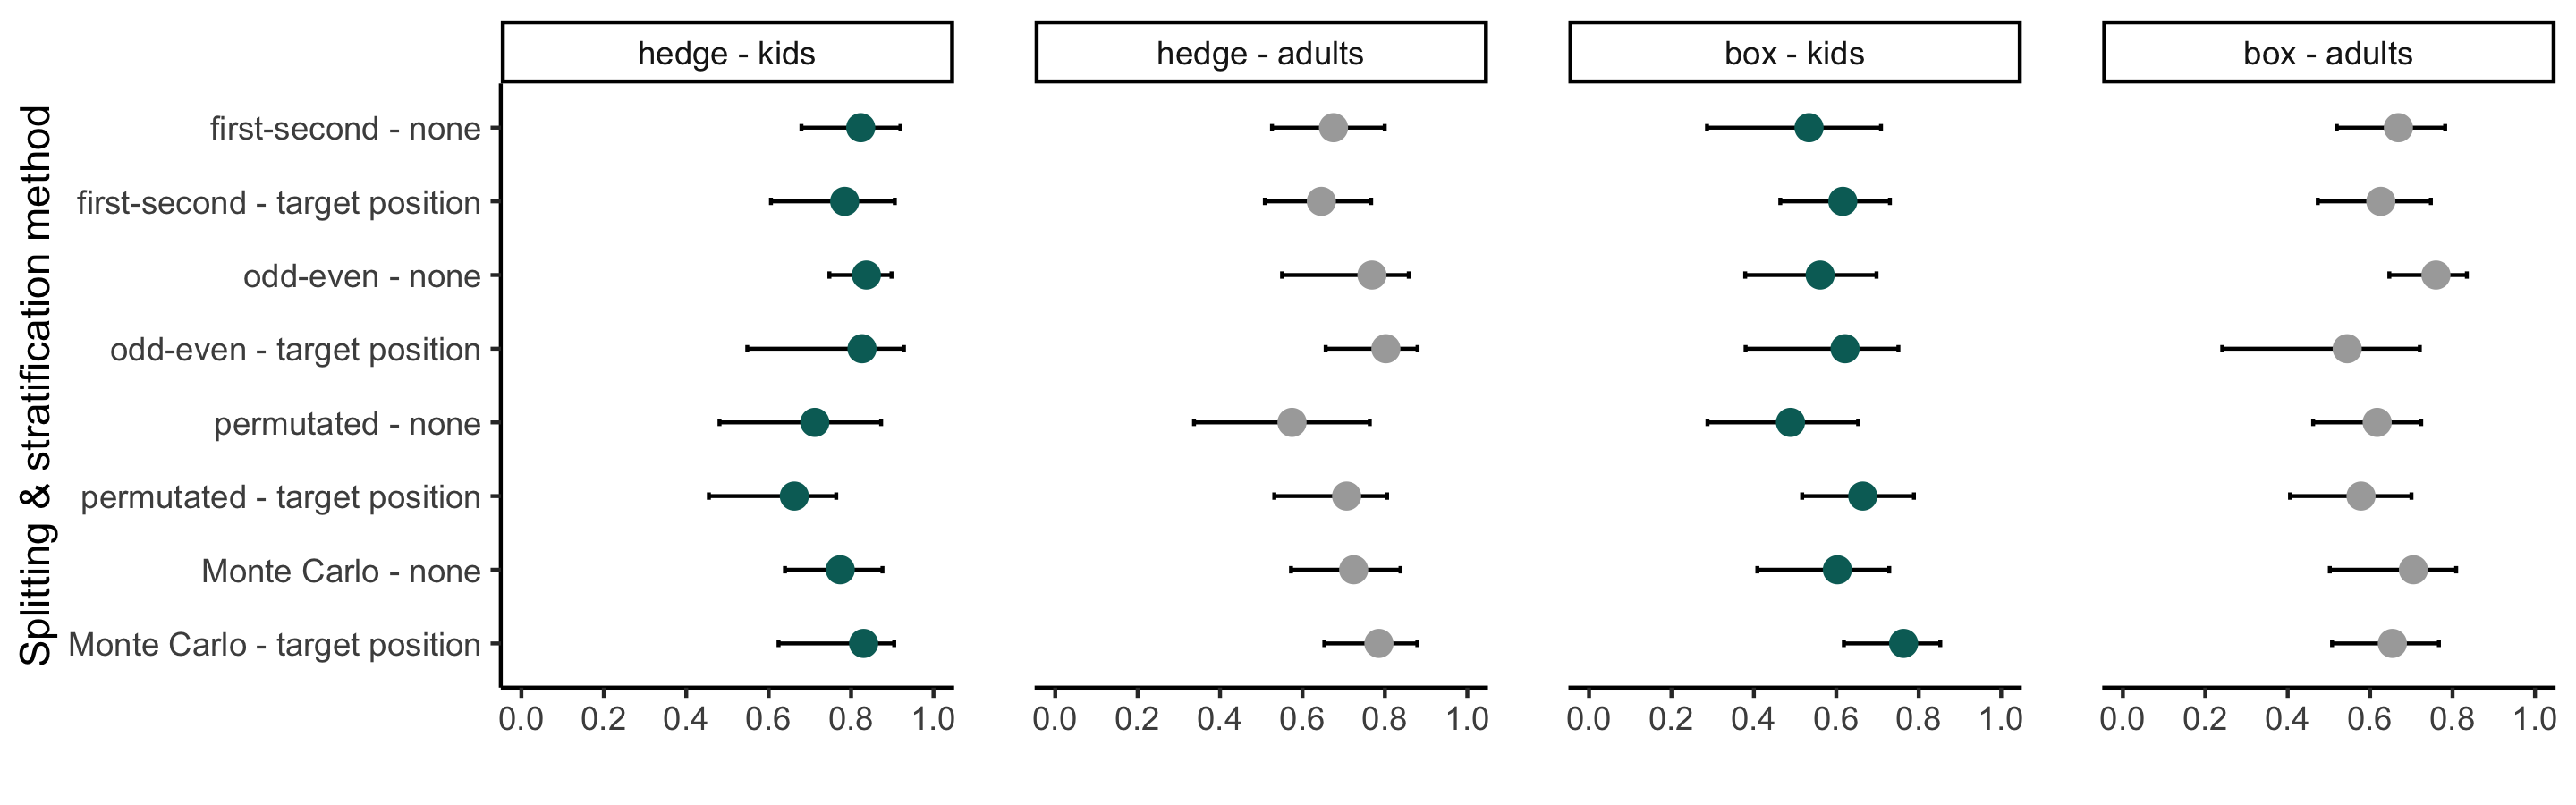
\includegraphics[width=1\linewidth]{../figures/gafo_splithalf} 

}

\caption{\textbf{Internal Consistency}.
Reliability coefficients per splitting method, stratification level, study version and age group. Error bars show the 95\% confidence intervals of the coefficient estimates, calculated with the function \texttt{by\_split} from the \texttt{splithalfr} package (Pronk et al., 2021).}\label{fig:fig3}
\end{figure}

For the test-retest reliability, we show the association between raw performance scores of the two test days and corresponding \emph{Pearson} correlation coefficients in Figure \ref{fig:fig2}D, E, I and J.\footnote{In the hedge version, we excluded one 5-year-old child from the test-retest analysis. The performance of the mentioned child was 3 standard deviations above the mean on both test days. Including the child yielded a \emph{Pearson} correlation coefficient of \emph{r} = 0.87.}

The age-corrected, GLMM based retest reliabilities for children yielded similar results. In hedge version it was 0.90 (95\% CI {[}0.68;1.00{]}).
In the box version it was 0.92 (95\% CI {[}0.70;1.00{]}).

\hypertarget{discussion-1}{%
\subsection{Discussion}\label{discussion-1}}

Our results indicated that the measured variation was systematic. As could be expected, the continuous measure of the hedge version yielded higher reliability estimates than the discrete box version. For children, the model based reliability estimates showed that the task did capture individual differences even when correcting for age. This corroborates what we already see in Figure \ref{fig:fig2}: there was a clear overlap between age groups, indicating that age is predictive of performance for the mean, but is not the main source of individual differences.

\hypertarget{validity}{%
\section{Validity}\label{validity}}

Our third aim was to assess whether the captured individual variation in gaze cue understanding relates to factors in children's real live social environment. Previous studies found associations between social cognition measures and various environmental factors (Devine \& Hughes, 2018; Hughes \& Leekam, 2004), including family background and education {[}Cutting and Dunn (1999); bulgarelli2016social{]}, number and age of siblings and family constellation Cassidy, Fineberg, Brown, \& Perkins (2005), interaction with siblings (Dunn et al., 1991), and centre-based childcare (Bulgarelli \& Molina, 2016). It is assumed that opportunities to play, communicate and argue with siblings and similarly-aged peers help children to understand the human mind. Therefore, if we find a link between gaze cue understanding and family factors, we regard this as an indicator for the predictive validity of our measure.

\hypertarget{participants-2}{%
\subsection{Participants}\label{participants-2}}

For this exploratory analysis, we included all children of the aforementioned samples where families filled out a short demographic questionnaire. This subsample consisted of
137 children, including
42 3-year-olds
(mean = 43.04 months,
SD = 3.25,
range = 36
- 47,
23 girls),
46 4-year-olds
(mean = 54.43 months,
SD = 2.76,
range = 48
- 59,
34 girls),
and 49 5-year-olds
(mean = 66.25 months,
SD = 3.47,
range = 60
- 71,
27 girls).

\hypertarget{procedure-2}{%
\subsection{Procedure}\label{procedure-2}}

Families of our kindergarten and online child sample were asked to fill out a brief demographic questionnaire. We asked for (1) the total number of household members, (2) the number of children, (3) age of the other children, (4) whether the child was in day care, and if yes, (5) since when and (6) for how long on an average day.

\hypertarget{analysis-2}{%
\subsection{Analysis}\label{analysis-2}}

To estimate the effects of social surrounding on gaze cue understanding, we fit GLMMs predicting the task performance by each of our questionnaire variables, controlling for age (in months, z-transformed), data collection mode (reference category: in-person supervised) and study version (reference category: hedge version). The models included random intercepts for each participant and each target position, and a random slope for symmetric target position within participants. Therefore, our null model closely resembled the structure from our first analysis (see Analysis section of \emph{Does the balloon finding task induce variation?}; here: \texttt{performance\ \textasciitilde{}\ age\ +\ datacollection\ +\ studyversion\ +\ (symmetricPosition\ \textbar{}\ subjID)\ +\ (1\ \textbar{}\ targetPosition)}).
In order to combine data of our two study versions, we transformed continuous click responses from the hedge version into a discrete outcome. For the target position, we categorized two adjacent bins as one imaginary box. To measure participants' performance, we created imaginary box boundaries around the target's landing position and examined whether the participant's click response fell into this imaginary box. Across the two study versions, we could consequently model the participant's correct response (0/1) using a \texttt{Bernoulli} distribution with a logit link function.
For model comparisons, we ran separate models, each with one of the following predictors as a fixed effects added to the null model: number of household members, number of children aged 0-18 in household, number of children aged 1-12 in household, hours spent in childcare each day, and age when subject entered childcare.
In addition, we calculated three index scores. First, we calculated a sibling variety score according to Candida C. Peterson (2000). Second, we implemented the modified version of Cassidy et al. (2005) (for more details, see Supplements). Third, based on our own data exploration, we calculated the amount of peer exposure determined as the number of siblings and the average hours spent in childcare (both z-transformed).
We compared the models using WAIC (widely applicable information criterion) scores and weights (McElreath, 2020). As an indicator of out-of-sample predictive accuracy, lower WAIC scores stand for a better model fit. WAIC weights represent the probability that the model in question provides the best out-of-sample prediction compared to the other models.

\hypertarget{results-2}{%
\subsection{Results}\label{results-2}}

The model including our peer exposure index, as defined as the number of other children in the household and average hours spent in childcare, showed the best out-of-sample predictive accuracy. Note that we did not find a great difference in WAIC scores between the compared models (see Supplements for WAIC scores and weights). The model estimates were all considerably smaller than estimates of age, study version and data collection, and all 95\% CIs included zero. For example, for our winning model, we found a peer exposure estimate of \(\beta\) =
0.17 (95\% CI {[}-0.03; 0.36{]}),
with the estimates of age being \(\beta\) =0.57 (95\% CI {[}0.38; 0.77{]}), data collection mode being \(\beta\) =0.95 (95\% CI {[}0.56; 1.35{]}), and study version \(\beta\) =1.87 (95\% CI {[}0.25; 3.59{]}). Nevertheless, a general pattern emerges: exposure to a more variable social environment positively influenced children's gaze cue understanding. The number of people and, more specifically, children, as well as the more diverse their age, the more likely children were to understand the agent's gaze cue. The only predictor resulting in a negative estimate was the age at which a participant entered childcare, i.e., the later a child entered, the better performance in the task.




\begin{figure}

{\centering 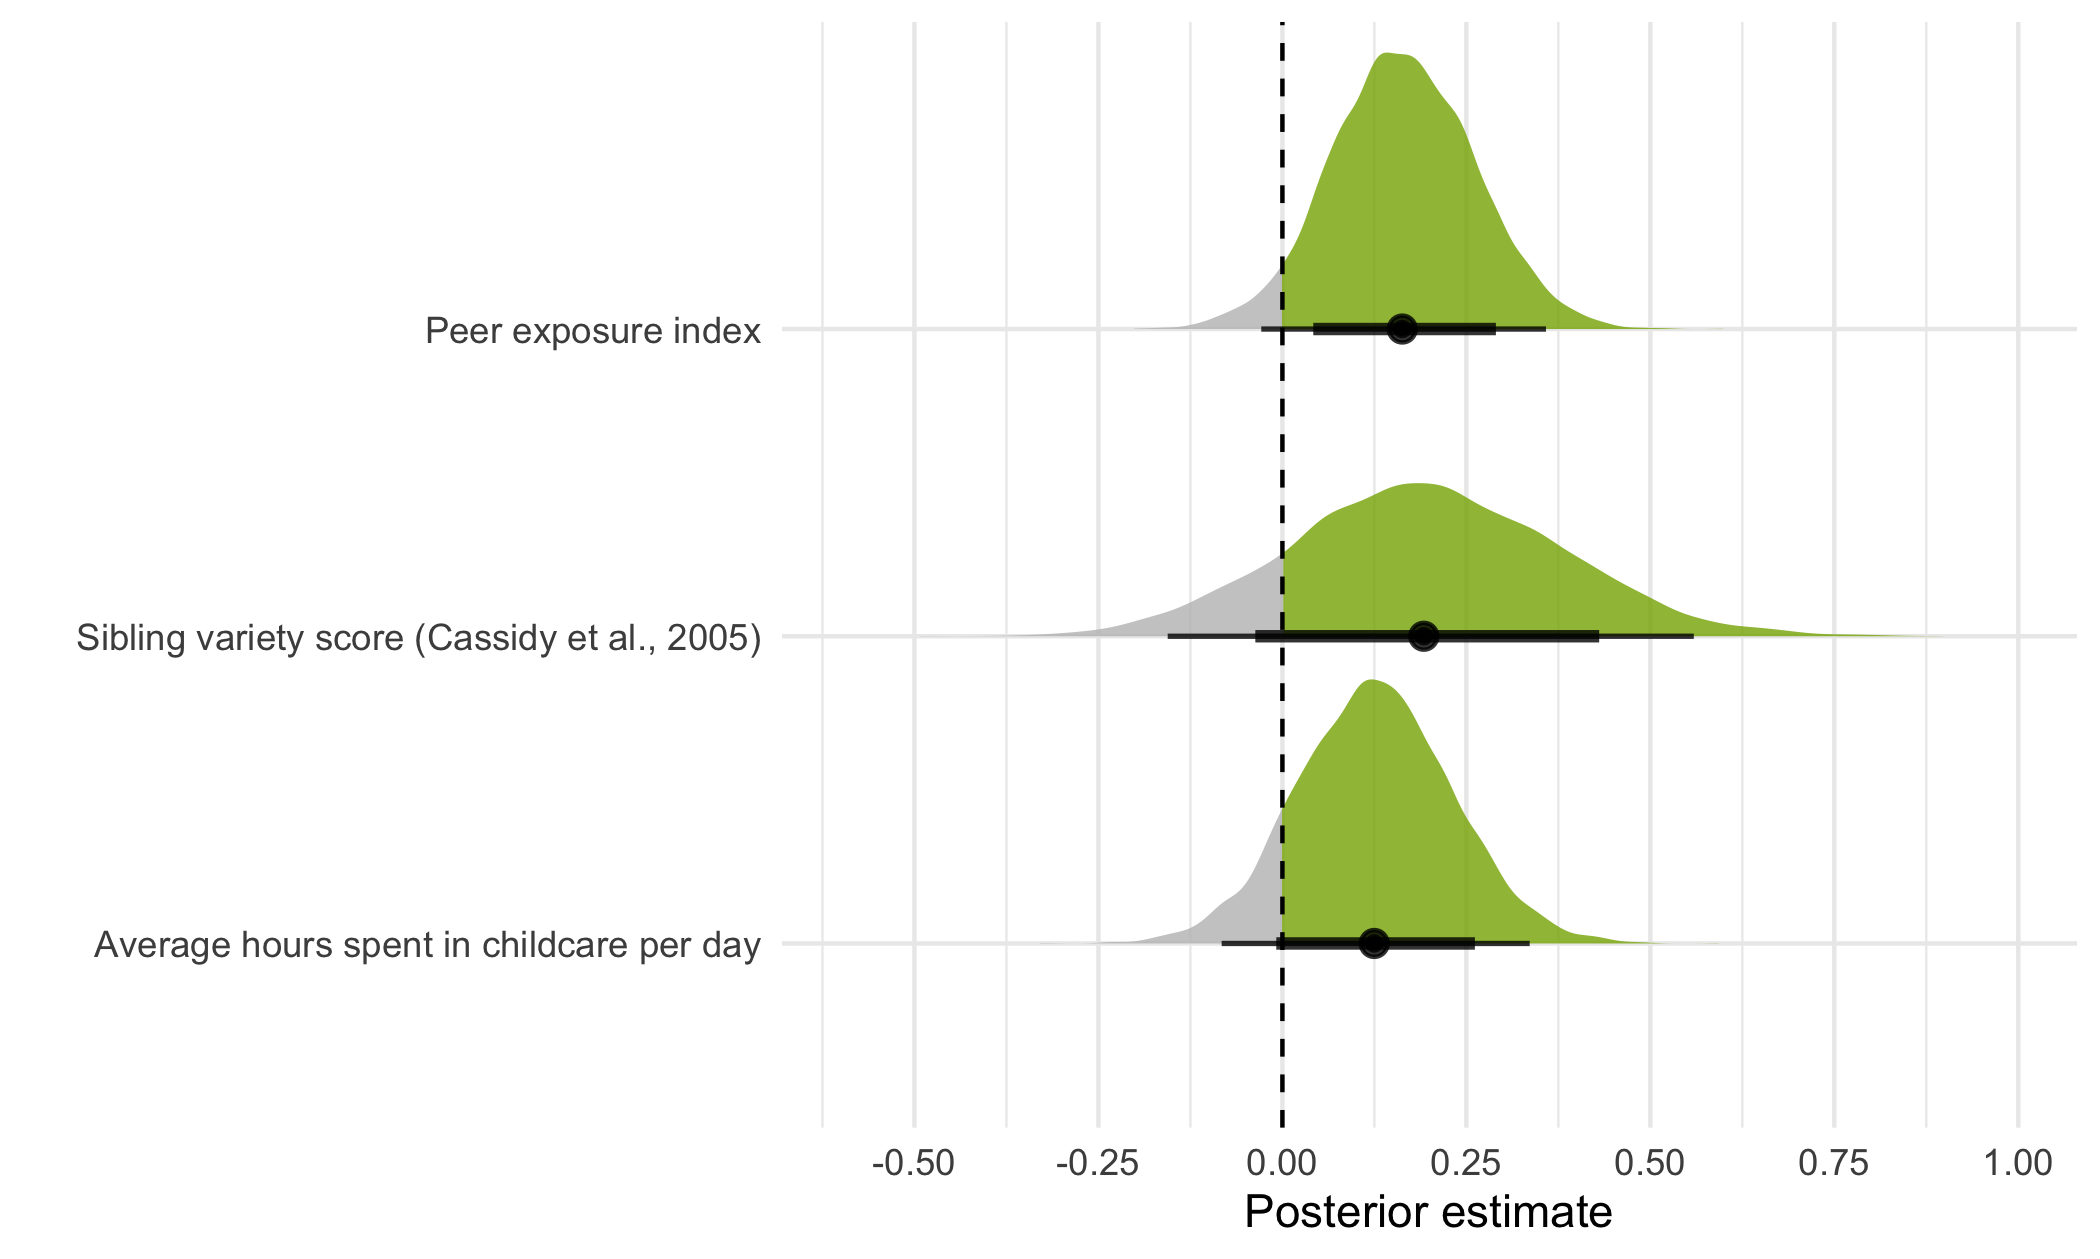
\includegraphics[width=1\linewidth]{../figures/extvali_results} 

}

\caption{\textbf{External validity of the balloon finding task}.
Factors of children's social surroundings and their influence on the probability of responding correctly. Models are ordered according to their WAIC scores, with the uppermost winning the model comparison. The graph shows the estimated density curves of a model's predictor coefficient. Only models performing better than our null model are included in the graph.}\label{fig:fig4}
\end{figure}

\hypertarget{discussion-2}{%
\subsection{Discussion}\label{discussion-2}}

We found that factors of children's social surrounding influenced their gaze cue understanding. Even though the effects are small and confidence intervals wide, it is remarkable that we were able to detect relationships between this fundamental social-cognitive ability and very distant, real life variables. Previous studies often focused on more complex, later developing social-cognitive abilities (e.g., false belief understanding). Apparently, systematic links between family factors and social-cognitive abilities can be found even when looking at more fundamental social-cognitive abilities like gaze cue understanding.

\hypertarget{discussion-3}{%
\section{Discussion}\label{discussion-3}}

We were able to show that our balloon finding task measures inter-individual variation between children and adults, alike. Our results suggest that the measured variation is systematic during the course of the same and different test days. Impressively, gaze cue understanding as measured by our task related to factors in children's everyday life experience.

\begin{itemize}
\tightlist
\item
  benefits of hedge (psychometric properties) vs box (discrete, easier for kids to click, induce salience etc)
\end{itemize}

\hypertarget{limitations}{%
\subsection{Limitations}\label{limitations}}

\hypertarget{future-development-extending-the-task}{%
\subsection{Future development / extending the task}\label{future-development-extending-the-task}}

\begin{itemize}
\tightlist
\item
  benefits of task battery
\end{itemize}

\hypertarget{conclusion}{%
\section{Conclusion}\label{conclusion}}

\hypertarget{declarations}{%
\section{Declarations}\label{declarations}}

\hypertarget{open-practices-statement}{%
\subsection{Open practices statement}\label{open-practices-statement}}

The web application (\url{https://ccp-odc.eva.mpg.de/gafo-demo/}) described here is open source (\url{https://github.com/ccp-eva/gafo-demo}).
The datasets generated during and/or analysed during the current study are available in the {[}gazecues-methods{]} repository, (\url{https://github.com/jprein/gazecues-methods}). All experiments were preregistered (\url{https://osf.io/zjhsc/}).

\hypertarget{funding}{%
\subsection{Funding}\label{funding}}

This study was funded by the Max Planck Society for the Advancement of Science, a noncommercial, publicly financed scientific organization (no grant number). We thank all the children and parents who participated in the study.

\hypertarget{conflicts-of-interest}{%
\subsection{Conflicts of interest}\label{conflicts-of-interest}}

The authors declare that they have no conflict of interest.

\hypertarget{ethics-approval}{%
\subsection{Ethics approval}\label{ethics-approval}}

\hypertarget{consent-to-participate}{%
\subsection{Consent to participate}\label{consent-to-participate}}

Informed consent was obtained from all individual participants included in the study or their legal guardians.

\hypertarget{consent-for-publication}{%
\subsection{Consent for publication}\label{consent-for-publication}}

\hypertarget{open-access}{%
\subsection{Open access}\label{open-access}}

\hypertarget{authors-contributions}{%
\subsection{Authors' contributions}\label{authors-contributions}}

optional: please review the submission guidelines from the journal whether statements are mandatory

\newpage

\hypertarget{references}{%
\section{References}\label{references}}

\begingroup
\setlength{\parindent}{-0.5in}
\setlength{\leftskip}{0.5in}

\hypertarget{refs}{}
\begin{CSLReferences}{1}{0}
\leavevmode\vadjust pre{\hypertarget{ref-astor2020social}{}}%
Astor, K., Lindskog, M., Forssman, L., Kenward, B., Fransson, M., Skalkidou, A., \ldots{} Gredebäck, G. (2020). Social and emotional contexts predict the development of gaze following in early infancy. \emph{Royal Society Open Science}, \emph{7}(9), 201178. \url{https://doi.org/10.1098/rsos.201178}

\leavevmode\vadjust pre{\hypertarget{ref-astor2021gaze}{}}%
Astor, K., Thiele, M., \& Gredebäck, G. (2021). Gaze following emergence relies on both perceptual cues and social awareness. \emph{Cognitive Development}, \emph{60}, 101121. \url{https://doi.org/10.1016/j.cogdev.2021.101121}

\leavevmode\vadjust pre{\hypertarget{ref-baron-cohen1985does}{}}%
Baron-Cohen, S., Leslie, A. M., \& Frith, U. (1985). Does the autistic child have a "theory of mind" ? \emph{Cognition}, \emph{21}, 37--46. \url{https://doi.org/10.1016/0010-0277(85)90022-8}

\leavevmode\vadjust pre{\hypertarget{ref-barrett2013early}{}}%
Barrett, H. C., Broesch, T., Scott, R. M., He, Z., Baillargeon, R., Wu, D., \ldots{} Laurence, S. (2013). Early false-belief understanding in traditional non-{Western} societies. \emph{Proceedings of the Royal Society B: Biological Sciences}. \url{https://doi.org/10.1098/rspb.2012.2654}

\leavevmode\vadjust pre{\hypertarget{ref-bartsch1996individual}{}}%
Bartsch, K., \& Estes, D. (1996). Individual differences in children's developing theory of mind and implications for metacognition. \emph{Learning and Individual Differences}, \emph{8}(4), 281--304. \url{https://doi.org/10.1016/S1041-6080(96)90020-5}

\leavevmode\vadjust pre{\hypertarget{ref-beaudoin2020systematic}{}}%
Beaudoin, C., Leblanc, É., Gagner, C., \& Beauchamp, M. H. (2020). Systematic {Review} and {Inventory} of {Theory} of {Mind Measures} for {Young Children}. \emph{Frontiers in Psychology}, \emph{0}. \url{https://doi.org/10.3389/fpsyg.2019.02905}

\leavevmode\vadjust pre{\hypertarget{ref-benson2012individual}{}}%
Benson, J., Sabbagh, M., Carlson, S., \& Zelazo, P. (2012). Individual {Differences} in {Executive Functioning Predict Preschoolers}' {Improvement From Theory-of-Mind Training}. \emph{Developmental Psychology}, \emph{49}. \url{https://doi.org/10.1037/a0031056}

\leavevmode\vadjust pre{\hypertarget{ref-brooks2005development}{}}%
Brooks, R., \& Meltzoff, A. N. (2005). The development of gaze following and its relation to language. \emph{Developmental Science}, \emph{8}(6), 535--543. \url{https://doi.org/10.1111/j.1467-7687.2005.00445.x}

\leavevmode\vadjust pre{\hypertarget{ref-bulgarelli2016social}{}}%
Bulgarelli, D., \& Molina, P. (2016). Social {Cognition} in {Preschoolers}: {Effects} of {Early Experience} and {Individual Differences}. \emph{Frontiers in Psychology}, \emph{7}. \url{https://doi.org/10.3389/fpsyg.2016.01762}

\leavevmode\vadjust pre{\hypertarget{ref-burkner2017brms}{}}%
Bürkner, P.-C. (2017). Brms: {An R Package} for {Bayesian Multilevel Models Using Stan}. \emph{Journal of Statistical Software}, \emph{80}(1). \url{https://doi.org/10.18637/jss.v080.i01}

\leavevmode\vadjust pre{\hypertarget{ref-burkner2018advanced}{}}%
Bürkner, P.-C. (2018). Advanced {Bayesian Multilevel Modeling} with the {R Package} brms. \emph{The R Journal}, \emph{10}(1), 395. \url{https://doi.org/10.32614/RJ-2018-017}

\leavevmode\vadjust pre{\hypertarget{ref-buttelmann2021relations}{}}%
Buttelmann, D., Kühn, K., \& Zmyj, N. (2021). The {Relations} among {Theory} of {Mind}, {Inhibitory Control}, and {Aggressive Behavior} in 4-{Year-Old Children} \textendash{} {A Multi-Measure Multi-Informant Approach}. \emph{Journal of Cognition and Development}, \emph{0}(0), 1--24. \url{https://doi.org/10.1080/15248372.2021.1987240}

\leavevmode\vadjust pre{\hypertarget{ref-byers-heinlein2021development}{}}%
Byers-Heinlein, K., Tsui, R. K.-Y., van Renswoude, D., Black, A. K., Barr, R., Brown, A., \ldots{} Singh, L. (2021). The development of gaze following in monolingual and bilingual infants: {A} multi-laboratory study. \emph{Infancy}, \emph{26}(1), 4--38. \url{https://doi.org/10.1111/infa.12360}

\leavevmode\vadjust pre{\hypertarget{ref-callaghan2005synchrony}{}}%
Callaghan, T., Rochat, P., Lillard, A., Claux, M. L., Odden, H., Itakura, S., \ldots{} Singh, S. (2005). Synchrony in the onset of mental-state reasoning: {Evidence} from five cultures. \emph{Psychological Science}. \url{https://doi.org/10.1111/j.0956-7976.2005.01544.x}

\leavevmode\vadjust pre{\hypertarget{ref-carlson2001individual}{}}%
Carlson, Stephanie M., \& Moses, L. J. (2001). Individual {Differences} in {Inhibitory Control} and {Children}'s {Theory} of {Mind}. \emph{Child Development}, \emph{72}(4), 1032--1053.

\leavevmode\vadjust pre{\hypertarget{ref-carlson2004individual}{}}%
Carlson, Stephanie M., Moses, L. J., \& Claxton, L. J. (2004). Individual differences in executive functioning and theory of mind: {An} investigation of inhibitory control and planning ability. \emph{Journal of Experimental Child Psychology}, \emph{87}(4), 299--319. \url{https://doi.org/10.1016/j.jecp.2004.01.002}

\leavevmode\vadjust pre{\hypertarget{ref-cassidy2005theory}{}}%
Cassidy, K. W., Fineberg, D. S., Brown, K., \& Perkins, A. (2005). Theory of {Mind May Be Contagious}, but {You Don}'t {Catch It} from {Your Twin}. \emph{Child Development}, \emph{76}(1), 97--106.

\leavevmode\vadjust pre{\hypertarget{ref-coelho2006searching}{}}%
Coelho, E., George, N., Conty, L., Hugueville, L., \& Tijus, C. (2006). Searching for asymmetries in the detection of gaze contact versus averted gaze under different head views: A behavioural study. \emph{Spatial Vision}, \emph{19}(6), 529--545. \url{https://doi.org/10.1163/156856806779194026}

\leavevmode\vadjust pre{\hypertarget{ref-cutting1999theory}{}}%
Cutting, A. L., \& Dunn, J. (1999). Theory of {Mind}, {Emotion Understanding}, {Language}, and {Family Background}: {Individual Differences} and {Interrelations}. \emph{Child Development}, \emph{70}(4), 853--865. \url{https://doi.org/10.1111/1467-8624.00061}

\leavevmode\vadjust pre{\hypertarget{ref-delbianco2019developmental}{}}%
Del Bianco, T., Falck-Ytter, T., Thorup, E., \& Gredebäck, G. (2019). The {Developmental Origins} of {Gaze-Following} in {Human Infants}. \emph{Infancy}, \emph{24}(3), 433--454. \url{https://doi.org/10.1111/infa.12276}

\leavevmode\vadjust pre{\hypertarget{ref-devine2018family}{}}%
Devine, R. T., \& Hughes, C. (2018). Family {Correlates} of {False Belief Understanding} in {Early Childhood}: {A Meta-Analysis}. \emph{Child Development}, \emph{89}(3), 971--987. \url{https://doi.org/10.1111/cdev.12682}

\leavevmode\vadjust pre{\hypertarget{ref-dunn1991young}{}}%
Dunn, J., Brown, J., Slomkowski, C., Tesla, C., \& Youngblade, L. (1991). \href{https://www.ncbi.nlm.nih.gov/pubmed/1786720}{Young children's understanding of other people's feelings and beliefs: Individual differences and their antecedents}. \emph{Child Development}, \emph{62}(6), 1352--1366.

\leavevmode\vadjust pre{\hypertarget{ref-frischen2007gaze}{}}%
Frischen, A., Bayliss, A. P., \& Tipper, S. P. (2007). Gaze cueing of attention: {Visual} attention, social cognition, and individual differences. \emph{Psychological Bulletin}, \emph{133}(4), 694--724. \url{https://doi.org/10.1037/0033-2909.133.4.694}

\leavevmode\vadjust pre{\hypertarget{ref-gola2012mental}{}}%
Gola, A. A. H. (2012). Mental verb input for promoting children's theory of mind: {A} training study. \emph{Cognitive Development}, \emph{27}(1), 64--76. \url{https://doi.org/10.1016/j.cogdev.2011.10.003}

\leavevmode\vadjust pre{\hypertarget{ref-gopnik1991young}{}}%
Gopnik, A., \& Slaughter, V. (1991). Young {Children}'s {Understanding} of {Changes} in {Their Mental States}. \emph{Child Development}, \emph{62}(1), 98. \url{https://doi.org/10.2307/1130707}

\leavevmode\vadjust pre{\hypertarget{ref-happe2017structure}{}}%
Happé, F., Cook, J. L., \& Bird, G. (2017). The {Structure} of {Social Cognition}: {In}(ter)dependence of {Sociocognitive Processes}. \emph{Annual Review of Psychology}, \emph{68}(1), 243--267. \url{https://doi.org/10.1146/annurev-psych-010416-044046}

\leavevmode\vadjust pre{\hypertarget{ref-hedge2018reliability}{}}%
Hedge, C., Powell, G., \& Sumner, P. (2018). The reliability paradox: {Why} robust cognitive tasks do not produce reliable individual differences. \emph{Behavior Research Methods}, \emph{50}(3), 1166--1186. \url{https://doi.org/10.3758/s13428-017-0935-1}

\leavevmode\vadjust pre{\hypertarget{ref-hernik2019infant}{}}%
Hernik, M., \& Broesch, T. (2019). Infant gaze following depends on communicative signals: {An} eye-tracking study of 5- to 7-month-olds in {Vanuatu}. \emph{Developmental Science}, \emph{22}(4), e12779. \url{https://doi.org/10.1111/desc.12779}

\leavevmode\vadjust pre{\hypertarget{ref-herrmann2010structure}{}}%
Herrmann, E., Hernández-Lloreda, M. V., Call, J., Hare, B., \& Tomasello, M. (2010). The {Structure} of {Individual Differences} in the {Cognitive Abilities} of {Children} and {Chimpanzees}. \emph{Psychological Science}, \emph{21}(1), 102--110. \url{https://doi.org/10.1177/0956797609356511}

\leavevmode\vadjust pre{\hypertarget{ref-hughes2000good}{}}%
Hughes, C., Adlam, A., Happé, F., Jackson, J., Taylor, A., \& Caspi, A. (2000). Good {Test}-{Retest Reliability} for {Standard} and {Advanced False}-{Belief Tasks} across a {Wide Range} of {Abilities}. \emph{Journal of Child Psychology and Psychiatry}, \emph{41}(4), 483--490. \url{https://doi.org/10.1111/1469-7610.00633}

\leavevmode\vadjust pre{\hypertarget{ref-hughes2015individual}{}}%
Hughes, C., \& Devine, R. T. (2015). Individual {Differences} in {Theory} of {Mind From Preschool} to {Adolescence}: {Achievements} and {Directions}. \emph{Child Development Perspectives}, \emph{9}(3), 149--153. \url{https://doi.org/10.1111/cdep.12124}

\leavevmode\vadjust pre{\hypertarget{ref-hughes2007executive}{}}%
Hughes, C., \& Ensor, R. (2007). Executive function and theory of mind: {Predictive} relations from ages 2 to 4. \emph{Developmental Psychology}, \emph{43}(6), 1447--1459. \url{https://doi.org/10.1037/0012-1649.43.6.1447}

\leavevmode\vadjust pre{\hypertarget{ref-hughes2011individual}{}}%
Hughes, C., Ensor, R., \& Marks, A. (2011). Individual differences in false belief understanding are stable from 3 to 6 years of age and predict children's mental state talk with school friends. \emph{Journal of Experimental Child Psychology}, \emph{108}(1), 96--112. \url{https://doi.org/10.1016/j.jecp.2010.07.012}

\leavevmode\vadjust pre{\hypertarget{ref-hughes2004links}{}}%
Hughes, C., \& Leekam, S. (2004). What are the {Links Between Theory} of {Mind} and {Social Relations}? {Review}, {Reflections} and {New Directions} for {Studies} of {Typical} and {Atypical Development}. \emph{Social Development}, \emph{13}(4), 590--619. \url{https://doi.org/10.1111/j.1467-9507.2004.00285.x}

\leavevmode\vadjust pre{\hypertarget{ref-imuta2016theory}{}}%
Imuta, K., Henry, J. D., Slaughter, V., Selcuk, B., \& Ruffman, T. (2016). Theory of mind and prosocial behavior in childhood: {A} meta-analytic review. \emph{Developmental Psychology}, \emph{52}(8), 1192--1205. \url{https://doi.org/10.1037/dev0000140}

\leavevmode\vadjust pre{\hypertarget{ref-itakura1998use}{}}%
Itakura, S., \& Tanaka, M. (1998). Use of experimenter-given cues during object-choice tasks by chimpanzees ({Pan} troglodytes), an orangutan ({Pongo} pygmaeus), and human infants ({Homo} sapiens). \emph{Journal of Comparative Psychology}, \emph{112}(2), 119--126. \url{https://doi.org/10.1037/0735-7036.112.2.119}

\leavevmode\vadjust pre{\hypertarget{ref-keenan2003individual}{}}%
Keenan, T. (2003). Individual {Differences} in {Theory} of {Mind}: {The Preschool Years} and {Beyond}. In \emph{Individual {Differences} in {Theory} of {Mind}}. {Psychology Press}.

\leavevmode\vadjust pre{\hypertarget{ref-kidd2018individual}{}}%
Kidd, E., Donnelly, S., \& Christiansen, M. H. (2018). Individual {Differences} in {Language Acquisition} and {Processing}. \emph{Trends in Cognitive Sciences}, \emph{22}(2), 154--169. \url{https://doi.org/10.1016/j.tics.2017.11.006}

\leavevmode\vadjust pre{\hypertarget{ref-lecce2014promoting}{}}%
Lecce, S., Bianco, F., Devine, R. T., Hughes, C., \& Banerjee, R. (2014). Promoting theory of mind during middle childhood: {A} training program. \emph{Journal of Experimental Child Psychology}, \emph{126}, 52--67. \url{https://doi.org/10.1016/j.jecp.2014.03.002}

\leavevmode\vadjust pre{\hypertarget{ref-lee1998children}{}}%
Lee, K., Eskritt, M., Symons, L. A., \& Muir, D. (1998). Children's use of triadic eye gaze information for "mind reading". \emph{Developmental Psychology}, \emph{34}(3), 525--539. \url{https://doi.org/10.1037//0012-1649.34.3.525}

\leavevmode\vadjust pre{\hypertarget{ref-mayer2015weird}{}}%
Mayer, A., \& Träuble, B. (2015). The weird world of cross-cultural false-belief research: {A} true- and false-belief study among samoan children based on commands. \emph{Journal of Cognition and Development}, \emph{16}(4), 650--665. \url{https://doi.org/10.1080/15248372.2014.926273}

\leavevmode\vadjust pre{\hypertarget{ref-mayes1996testretest}{}}%
Mayes, L. C., Klin, A., Tercyak, K. P., Cicchetti, D. V., \& Cohen, D. J. (1996). Test-{Retest Reliability} for {False-Belief Tasks}. \emph{Journal of Child Psychology and Psychiatry}, \emph{37}(3), 313--319. \url{https://doi.org/10.1111/j.1469-7610.1996.tb01408.x}

\leavevmode\vadjust pre{\hypertarget{ref-mcelreath2020statistical}{}}%
McElreath, R. (2020). \emph{Statistical rethinking: {A Bayesian Course} with {Examples} in {R} and {Stan}} (Second). {Chapman and Hall/CRC}.

\leavevmode\vadjust pre{\hypertarget{ref-mcewen2007origins}{}}%
McEwen, F., Happé, F., Bolton, P., Rijsdijk, F., Ronald, A., Dworzynski, K., \& Plomin, R. (2007 Mar-Apr). Origins of individual differences in imitation: Links with language, pretend play, and socially insightful behavior in two-year-old twins. \emph{Child Development}, \emph{78}(2), 474--492. \url{https://doi.org/10.1111/j.1467-8624.2007.01010.x}

\leavevmode\vadjust pre{\hypertarget{ref-milligan2007language}{}}%
Milligan, K., Astington, J. W., \& Dack, L. A. (2007). Language and {Theory} of {Mind}: {Meta-Analysis} of the {Relation Between Language Ability} and {False-belief Understanding}. \emph{Child Development}, \emph{78}(2), 622--646. \url{https://doi.org/10.1111/j.1467-8624.2007.01018.x}

\leavevmode\vadjust pre{\hypertarget{ref-moore2008development}{}}%
Moore, C. (2008). The {Development} of {Gaze Following}. \emph{Child Development Perspectives}, \emph{2}(2), 66--70. \url{https://doi.org/10.1111/j.1750-8606.2008.00052.x}

\leavevmode\vadjust pre{\hypertarget{ref-mundy2007individual}{}}%
Mundy, P., Block, J., Delgado, C., Pomares, Y., Van Hecke, A. V., \& Parlade, M. V. (2007). Individual differences and the development of joint attention in infancy. \emph{Child Development}, \emph{78}(3), 938--954. \url{https://doi.org/10.1111/j.1467-8624.2007.01042.x}

\leavevmode\vadjust pre{\hypertarget{ref-okumura2017individual}{}}%
Okumura, Y., Kanakogi, Y., Kobayashi, T., \& Itakura, S. (2017). Individual differences in object-processing explain the relationship between early gaze-following and later language development. \emph{Cognition}, \emph{166}, 418--424. \url{https://doi.org/10.1016/j.cognition.2017.06.005}

\leavevmode\vadjust pre{\hypertarget{ref-palan2018prolific}{}}%
Palan, S., \& Schitter, C. (2018). Prolific.ac\textemdash{{A}} subject pool for online experiments. \emph{Journal of Behavioral and Experimental Finance}, \emph{17}, 22--27. \url{https://doi.org/10.1016/j.jbef.2017.12.004}

\leavevmode\vadjust pre{\hypertarget{ref-pavarini2013parental}{}}%
Pavarini, G., de Hollanda Souza, D., \& Hawk, C. K. (2013). Parental {Practices} and {Theory} of {Mind Development}. \emph{Journal of Child and Family Studies}, \emph{22}(6), 844--853. \url{https://doi.org/10.1007/s10826-012-9643-8}

\leavevmode\vadjust pre{\hypertarget{ref-perner1994theory}{}}%
Perner, J., Ruffman, T., \& Leekam, S. R. (1994). Theory of {Mind Is Contagious}: {You Catch It} from {Your Sibs}. \emph{Child Development}, \emph{65}(4), 1228--1238. \url{https://doi.org/10.2307/1131316}

\leavevmode\vadjust pre{\hypertarget{ref-peterson2000kindred}{}}%
Peterson, Candida C. (2000). Kindred spirits: {Influences} of siblings' perspectives on theory of mind. \emph{Cognitive Development}, \emph{15}(4), 435--455. \url{https://doi.org/10.1016/S0885-2014(01)00040-5}

\leavevmode\vadjust pre{\hypertarget{ref-peterson2012mind}{}}%
Peterson, Candida C., Wellman, H. M., \& Slaughter, V. (2012). The {Mind Behind} the {Message}: {Advancing Theory-of-Mind Scales} for {Typically Developing Children}, and {Those With Deafness}, {Autism}, or {Asperger Syndrome}: {\textbf{The Mind Behind}}{ \textbf{the} }{\textbf{Message}}. \emph{Child Development}, \emph{83}(2), 469--485. \url{https://doi.org/10.1111/j.1467-8624.2011.01728.x}

\leavevmode\vadjust pre{\hypertarget{ref-pronk2021methods}{}}%
Pronk, T., Molenaar, D., Wiers, R. W., \& Murre, J. (2021). Methods to split cognitive task data for estimating split-half reliability: {A} comprehensive review and systematic assessment. \emph{Psychonomic Bulletin \& Review}. \url{https://doi.org/10.3758/s13423-021-01948-3}

\leavevmode\vadjust pre{\hypertarget{ref-rcoreteam2022language}{}}%
R Core Team. (2022). \emph{R: {A} language and environment for statistical computing} {[}Manual{]}. {Vienna, Austria}: {R Foundation for Statistical Computing}.

\leavevmode\vadjust pre{\hypertarget{ref-rakoczy2022foundations}{}}%
Rakoczy, H. (2022). Foundations of theory of mind and its development in early childhood. \emph{Nature Reviews Psychology}, 1--13. \url{https://doi.org/10.1038/s44159-022-00037-z}

\leavevmode\vadjust pre{\hypertarget{ref-repacholi2004individual}{}}%
Repacholi, B., \& Slaughter, V. (Eds.). (2004). \emph{Individual {Differences} in {Theory} of {Mind}} (Zeroth). {New York}: {Psychology Press}. \url{https://doi.org/10.4324/9780203488508}

\leavevmode\vadjust pre{\hypertarget{ref-repacholi2003introduction}{}}%
Repacholi, V. S. \&. B. (2003). Introduction {Individual Differences} in {Theory} of {Mind}: {What Are We Investigating}? In \emph{Individual {Differences} in {Theory} of {Mind}}. {Psychology Press}.

\leavevmode\vadjust pre{\hypertarget{ref-rizzo2018theory}{}}%
Rizzo, M. T., \& Killen, M. (2018). Theory of mind is related to children's resource allocations in gender stereotypic contexts. \emph{Developmental Psychology}, \emph{54}(3), 510. \url{https://doi.org/10.1037/dev0000439}

\leavevmode\vadjust pre{\hypertarget{ref-rouder2019psychometrics}{}}%
Rouder, J. N., \& Haaf, J. M. (2019). A psychometrics of individual differences in experimental tasks. \emph{Psychonomic Bulletin \& Review}, \emph{26}(2), 452--467. \url{https://doi.org/10.3758/s13423-018-1558-y}

\leavevmode\vadjust pre{\hypertarget{ref-schaafsma2015deconstructing}{}}%
Schaafsma, S. M., Pfaff, D. W., Spunt, R. P., \& Adolphs, R. (2015). Deconstructing and reconstructing theory of mind. \emph{Trends in Cognitive Sciences}, \emph{19}(2), 65--72. \url{https://doi.org/10.1016/j.tics.2014.11.007}

\leavevmode\vadjust pre{\hypertarget{ref-shepherd2010following}{}}%
Shepherd, S. (2010). Following {Gaze}: {Gaze-Following Behavior} as a {Window} into {Social Cognition}. \emph{Frontiers in Integrative Neuroscience}, \emph{4}.

\leavevmode\vadjust pre{\hypertarget{ref-slaughter2015theorya}{}}%
Slaughter, V. (2015). Theory of {Mind} in {Infants} and {Young Children}: {A Review}. \emph{Australian Psychologist}, \emph{50}(3), 169--172. \url{https://doi.org/10.1111/ap.12080}

\leavevmode\vadjust pre{\hypertarget{ref-sodian2016understanding}{}}%
Sodian, B., Licata, M., Kristen-Antonow, S., Paulus, M., Killen, M., \& Woodward, A. (2016). Understanding of {Goals}, {Beliefs}, and {Desires Predicts Morally Relevant Theory} of {Mind}: {A Longitudinal Investigation}. \emph{Child Development}, \emph{87}(4), 1221--1232. \url{https://doi.org/10.1111/cdev.12533}

\leavevmode\vadjust pre{\hypertarget{ref-stenhaug2021structure}{}}%
Stenhaug, B., Ram, N., \& Frank, M. C. (2021). \emph{The {Structure} of {Developmental Variation} in {Early Childhood}}. {PsyArXiv}. \url{https://doi.org/10.31234/osf.io/95erq}

\leavevmode\vadjust pre{\hypertarget{ref-tomasello2007reliance}{}}%
Tomasello, M., Hare, B., Lehmann, H., \& Call, J. (2007). Reliance on head versus eyes in the gaze following of great apes and human infants: The cooperative eye hypothesis. \emph{Journal of Human Evolution}, \emph{52}(3), 314--320. \url{https://doi.org/10.1016/j.jhevol.2006.10.001}

\leavevmode\vadjust pre{\hypertarget{ref-underwood1975individual}{}}%
Underwood, B. J. (1975). Individual differences as a crucible in theory construction. \emph{American Psychologist}, \emph{30}(2), 128--134. \url{https://doi.org/10.1037/h0076759}

\leavevmode\vadjust pre{\hypertarget{ref-walker2005gender}{}}%
Walker, S. (2005). Gender {Differences} in the {Relationship Between Young Children}'s {Peer-Related Social Competence} and {Individual Differences} in {Theory} of {Mind}. \emph{The Journal of Genetic Psychology}, \emph{166}(3), 297--312. \url{https://doi.org/10.3200/GNTP.166.3.297-312}

\leavevmode\vadjust pre{\hypertarget{ref-wellman2012theory}{}}%
Wellman, H. M. (2012). Theory of mind: {Better} methods, clearer findings, more development. \emph{European Journal of Developmental Psychology}, \emph{9}(3), 313--330. \url{https://doi.org/10.1080/17405629.2012.680297}

\leavevmode\vadjust pre{\hypertarget{ref-zhang2021worse}{}}%
Zhang, Z., Yu, H., Long, M., \& Li, H. (2021). Worse {Theory} of {Mind} in {Only-Children Compared} to {Children With Siblings} and {Its Intervention}. \emph{Frontiers in Psychology}, \emph{12}, 5073. \url{https://doi.org/10.3389/fpsyg.2021.754168}

\end{CSLReferences}

\endgroup

\newpage

\hypertarget{supplements}{%
\section{Supplements}\label{supplements}}

\hypertarget{child-sample}{%
\subsection{Child sample}\label{child-sample}}

\hypertarget{webcam-coding}{%
\subsubsection{Webcam coding}\label{webcam-coding}}




\begin{figure}

{\centering 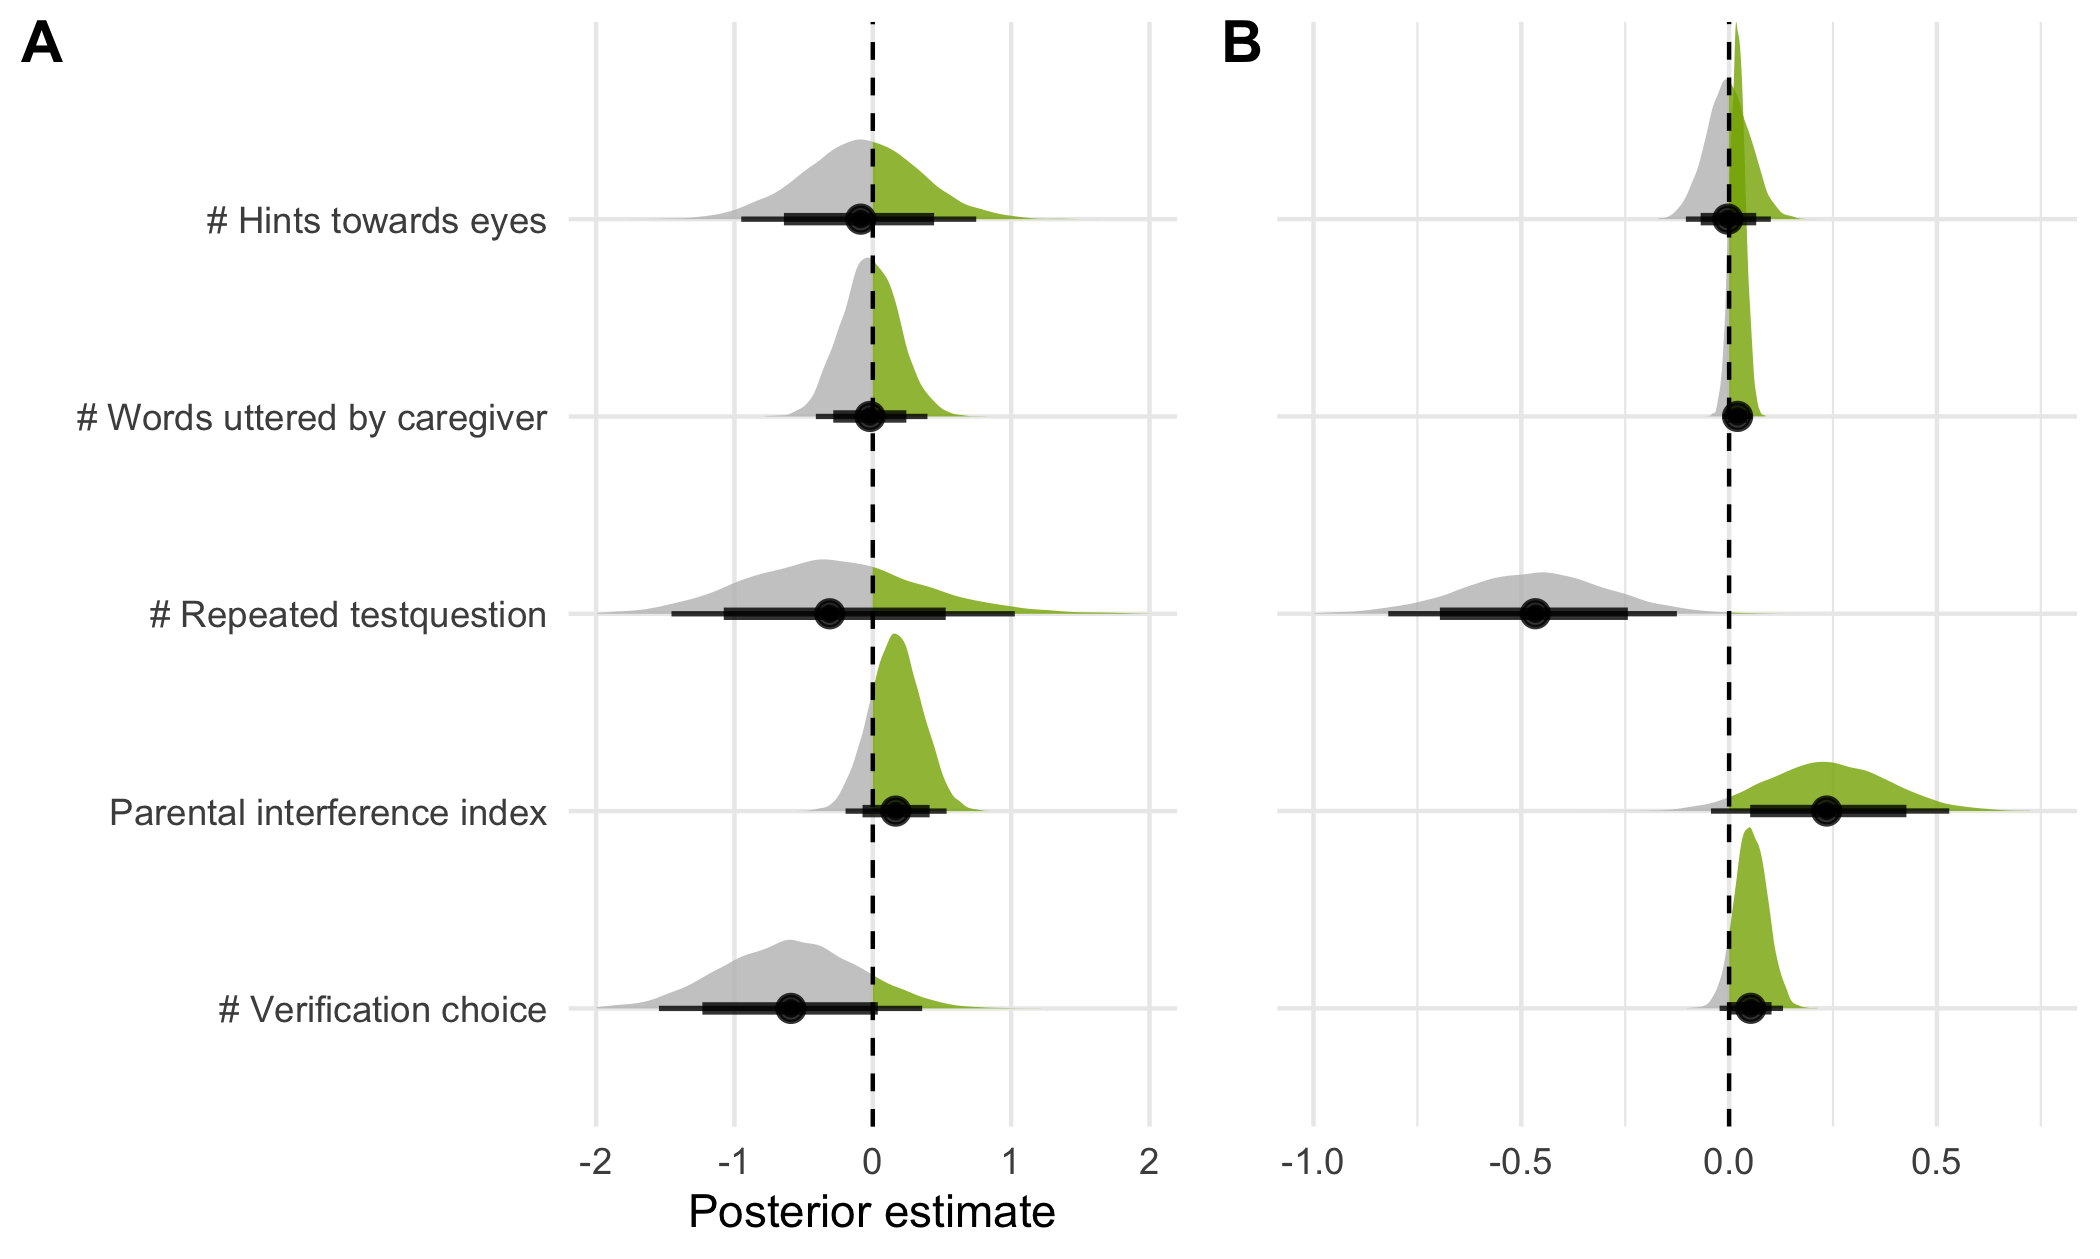
\includegraphics[width=1\linewidth]{../figures/supplements_webcamcoding_draws} 

}

\caption{\textbf{Model comparison for exploratory webcam coding of parental interference}.
Factors of parental interference and their influence on the probability of responding correctly. The graph shows the estimated density curves of a model's predictor coefficient. Models are ordered according to their WAIC scores in the trial-by-trial analysis, with the uppermost winning the model comparison. (A) Analysis on a trial-by-trial level. (B) Analysis on a subject level.}\label{fig:fig5}
\end{figure}

Comparing the performances of children across our two data collection modes, we found that children participating remotely were slightly more precise. This difference was especially prominent in younger participants in the box version of the task. It is conceivable that caregivers were especially prone to influence the behavior of younger children. In the box version, caregivers might have had more opportunities to interfere since they carried out the clicking for their children.
In an exploratory analysis, we coded parental behavior and environmental factors during remote unsupervised testing. Due to the time consuming nature of hand coding videos frame by frame, we focused on the subsample with the greatest performance difference between data collection modes: the three-year-olds in the box version of the task (n = 16). We reasoned that if parental interference cannot explain the greatest performance difference in our sample, the effects would be negligible in the remaining sample.
A trial was defined as the time between two eye blinking sounds. We transcribed all utterances by parents and children and counted the words uttered by each. We then classified the utterances into several categories: question asked by child, repeated test questions by caregiver, hints towards agents (how many times the caregivers guided the child's attention to the agent), hints towards eyes (how many times the caregivers guided the child's attention to the agent's eyes), verification of choice (how many times the caregiver questioned or double checked the child's response), mentioning of screen (how many times the caregiver verbally guided the child's attention to the screen), pointing to screen (how many times the caregiver pointed towards the screen), positive \& negative feedback, motivational statements, and incomprehensible utterances.
In addition, we coded how many adults and children were present, whether a response click was obviously conducted by the caregiver themselves, and whether children took a break during the trial.
We conducted a model comparison to estimate the effects of parental interference. Our null model explained the response behavior by age, while including random effects for subject and target position (model notation in \texttt{R:\ correct\ \textasciitilde{}\ age\ +\ (1\ \textbar{}\ subjID)\ +\ (1\ \textbar{}\ targetPosition)}.\footnote{Attentive readers might notice that we simplified the structure of random effects. Compared to our models in the \emph{Individual differences} and \emph{External Validity} sections, this model does not include the random slope for symmetric target position within participants. We decided to do so since we had limited amount of data from few participants.}

We compared this null model to models including the number of words uttered by the caregiver, number of repeated testquestions, verification of choice, or hints towards eyes as fixed effects. Furthermore, we calculated an parental interference index by summing up number of repeated testquestions, verification of choice, and hints towards eyes, with the sign matching the variable's direction of effect. Remaining variables that we coded for were not included since there was not enough variation and/or occurrences in our sample.
We compared models using WAIC (widely applicable information criterion) scores and weights. As an indicator of out-of-sample predictive accuracy, lower WAIC scores stand for a better model fit. WAIC weights represent the probability that the model in question provides the best out-of-sample prediction compared to the other models.
On the trial level, the model including the verification of choice as a main effect performed best: here, the less the caregivers asked for children's responses again, the more likely children clicked on the correct box. Interestingly, the effect reversed on a subject level - possibly due to greater learning effects for the children that were most likely to click incorrectly in the beginning and then receiving most parental comments. On the subject level, the model including number of repeated test questions performed best: the more caregivers asked again where the target landed, the more likely children were to respond to the incorrect box. In all cases, however, ELPD difference scores were smaller than their standard errors. Similarly, 95\% CI of the model estimates included zero and were rather wide (Table \ref{tab:webcam_table}). Therefore, we conclude that the effect of parental interference was negligable and could, most likely, be explained as described above.

\hypertarget{appendix-to-external-validity-section}{%
\subsubsection{Appendix to external validity section}\label{appendix-to-external-validity-section}}

\hypertarget{scoring-of-sibling-variety-scores}{%
\paragraph{Scoring of sibling variety scores}\label{scoring-of-sibling-variety-scores}}

For assessing the external validity of our balloon finding task, we calculated two sibling variety scores based on the existing Theory of Mind literature.
First, we followed the approach by Candida C. Peterson (2000). Here, only-children as well as firstborns with siblings under one year scored 0 points; lastborns with siblings above 12 years scored 0.5 points; children with twins, firstborns with siblings over one year, and lastborns with at least one sibling under 13 years scored 1 point, middleborns with at least one older and younger sibling aged one to 12 years scored 2 points.

Second, we implemented the sibling variety score by Cassidy et al. (2005). The authors adjusted the original score of Candida C. Peterson (2000) in the following way: only-children scored 0 points; children with a sibling under one year or above 12 years, and twins with no other sibling scored 0.5 points; children with a sibling above one year or under 13 years scored 1 point; middleborns with at least one older and younger sibling aged one to 12 years scored 2 points. Twins with additional siblings scored depending on the age and number of their siblings.

The reasoning was that children between one and 13 years of age would engage in sibling play, while the youngest and most mature siblings would be less likely to participate in such. However, teenage siblings might provide opportunities for interesting discussions (Candida C. Peterson, 2000).

\hypertarget{waic-scores-and-weights-of-the-model-comparison}{%
\paragraph{WAIC scores and weights of the model comparison}\label{waic-scores-and-weights-of-the-model-comparison}}

As can be seen, ELPD difference scores are smaller than their respective standard errors. WAIC scores between models don't differ substantially (Table \ref{tab:extvali_table}). All effects except when a child entered childcare positively influence performance.

\begin{table}[tbp]

\begin{center}
\begin{threeparttable}

\caption{\label{tab:extvali_table}Model comparison for influences of children's social surrounding}

\begin{tabular}{llllll}
\toprule
Predictor & \multicolumn{1}{c}{WAIC} & \multicolumn{1}{c}{SE\_WAIC} & \multicolumn{1}{c}{Weight} & \multicolumn{1}{c}{ELPD\_DIFF} & \multicolumn{1}{c}{SE\_ELPD\_DIFF}\\
\midrule
Average hours spent in childcare per day & 2,540.39 & 52.23 & 0.54 & 0.00 & 0.00\\
Peer exposure index & 2,541.00 & 52.22 & 0.28 & -0.30 & 0.92\\
\# Children in household aged 0-18 & 2,541.65 & 52.30 & 0.02 & -0.63 & 1.09\\
Sibling variety score (Cassidy et al., 2005) & 2,541.76 & 52.33 & 0.01 & -0.68 & 1.05\\
Sibling variety score (Peterson, 2000) & 2,541.80 & 52.38 & 0.02 & -0.71 & 1.10\\
Age of childcare entry & 2,542.19 & 52.38 & 0.12 & -0.90 & 1.32\\
\# Children in household aged 1-12 & 2,542.26 & 52.34 & 0.00 & -0.94 & 0.92\\
Null model & 2,542.58 & 52.26 & 0.00 & -1.09 & 0.79\\
\# Household members & 2,543.46 & 52.36 & 0.00 & -1.54 & 0.97\\
\bottomrule
\addlinespace
\end{tabular}

\begin{tablenotes}[para]
\normalsize{\textit{Note.} All models included random intercepts for each participant and each target position, and a random slope for symmetric target position within participants}
\end{tablenotes}

\end{threeparttable}
\end{center}

\end{table}

\hypertarget{adult-sample}{%
\subsection{Adult sample}\label{adult-sample}}

\hypertarget{recruitment}{%
\subsubsection{Recruitment}\label{recruitment}}

We recruited participants using the online participant recruitment service \emph{Prolific} from the University of Oxford. \emph{Prolific}'s subject pool consists of a mostly European and US-american sample although subjects from all over the world are included. The recruitment platform realises ethical payment of participants, which requires researchers to pay participants a fixed minimum wage of £5.00 (around US\$6.50 or €6.00) per hour. We decided to pay all participants the same fixed fee which was in relation to the estimated average time taken to complete the task.
\emph{Prolific} distributed our study link to potential participants, while the hosting of the online study was done by local servers in the Max Planck Institute for Evolutionary Anthropology, Leipzig. Therefore, study data was saved only on our internal servers, while \emph{Prolific} provided demographic information of the participants.
Participants' \emph{Prolific} ID was forwarded to our study website using URL parameters. This way, we could match participant demographic data to our study data. The same technique was used to confirm study completion: we redirected participants from our study website back to the \emph{Prolific} website using URL parameters.
We used \emph{Prolific}'s inbuilt prescreening filter to include only participants who were fluent in English and could therefore properly understand our written and oral study instructions.

\hypertarget{study-1---validation-hedge-version}{%
\subsubsection{Study 1 - Validation hedge version}\label{study-1---validation-hedge-version}}

The aim of Study 1 was to validate the hedge version of our balloon finding task. The pre-registration can be found here: \url{https://osf.io/r3bhn}. We recruited participants online by advertising the study on \emph{Prolific}.

50 adults participated in the study. One additional subject returned their submission, i.e., decided to leave the study early or withdrew their submission after study completion. Data collection took place in May 2021.
Participants were compensated with £1.25 for completing the study. We estimated an average completion time of 6 minutes, resulting in an estimated hourly rate of £10.00. In average, participants took 05:56min to complete the study.
Participants were required to complete the study on a tablet or desktop. Participation on mobile devices was disabled since the display would be too small and would harm click precision. It was indicated that the study required audio sound.

We stored \emph{Prolific}'s internal demographic information, while not asking for additional personal information.

\hypertarget{study-2---validation-box-version}{%
\subsubsection{Study 2 - Validation box version}\label{study-2---validation-box-version}}

As in study 1, we recruited participants on \emph{Prolific}, and employed the same methodology. However, this time we focussed on validating the box version of the task in an adult sample. Participants were presented with eight boxes in which the target could land.
50 adults participated in the study. One additional subject returned their submission, i.e., decided to leave the study early or withdrew their submission after study completion. Data collection took place in June 2021.
Participants were compensated with £1.00 for completing the study. We estimated an average completion time of 6 minutes, resulting in an estimated hourly rate of £10.00. In average, participants took 04:43min to complete the study.

\hypertarget{study-3---reliability-hedge-version}{%
\subsubsection{Study 3 - Reliability hedge version}\label{study-3---reliability-hedge-version}}

In study 3 and 4, we assessed the test-retest reliability of our balloon-finding task in an adult sample. The pre-registration can be found here: \url{https://osf.io/nu62m}. We tested the same participants twice with a delay of two weeks. The testing conditions were as specified in Study 1 and 2. However, the target locations as well as the succession of animals and target colors was randomized once. Each participant then received the same fixed randomized order of target location, animal, and target color. Participants received 30 test trials without voice-over description, so that each of the ten bins occurred exactly three times.

In addition to the beforementioned prescreening settings, we used a whitelist. \emph{Prolific} has a so-called \emph{custom allowlist prescreening filter} where one can enter the \emph{Prolific} IDs of participants who completed a previous study. Only these subjects are then invited to participate in a study. This way, repeated measurements can be implemented, collecting data from the same subjects at different points in time.

In a first round, 60 participants took part on the first testday. Additional two subjects returned their submission, i.e., decided to leave the study early or withdrew their submission after study completion. One additional participant timed out, i.e., did not finish the survey within the allowed maximum time. The maximum time is calculated by \emph{Prolific}, based on the estimated average completion time. For this study, the maximum time amounted to 41 minutes. For the first testday, participants were compensated with £1.25. We estimated an average completion time of 9 minutes, resulting in an estimated hourly rate of £8.33. In average, participants took 07:11min to complete the first part.

Of the 60 participants that completed testday 1, 41 subjects finished testday 2. One additional participant timed out, i.e., did not finish the survey within the allowed maximum time. Participants were compensated with £1.50 for completing the second part of the study. We estimated an average completion time of 9 minutes, resulting in an estimated hourly rate of £10. In average, participants took 06:36min to complete the second part of the study.

Since we aimed for a minimum sample size of 60 subjects participating on both testdays, we reran the first testday with additional 50 participants. Additional seven subjects returned their submission, i.e., decided to leave the study early or withdrew their submission after study completion. Two additional participants timed out, i.e., did not finish the survey within the allowed maximum time. Again, participants were compensated with £1.25 for completing the first part of the study (estimated average completion time 9 minutes, estimated hourly rate of £8.33). In average, participants took 06:51min to complete the first part.

Of the additional 50 participants that completed testday 1, 29 subjects finished testday 2. Again, participants were compensated with £1.50 for completing the second part of the study (estimated average completion time 9 minutes, estimated hourly rate of £10). In average, participants took 06:26min to complete the second part of the study.

\hypertarget{study-4---reliability-box-version}{%
\subsubsection{Study 4 - Reliability box version}\label{study-4---reliability-box-version}}

As in study 3, we recruited participants on \emph{Prolific}, and employed the same methodology. However, this time participants were presented with the box version of the task. Participants received 32 test trials without voice-over description, so that each of the eight boxes occurred exactly four times. As in study 2, we employed eight boxes in which the target could land.

In a first round, 60 participants took part on the first testday. Additional five subjects returned their submission, i.e., decided to leave the study early or withdrew their submission after study completion. For the first testday, participants were compensated with £1.25. We estimated an average completion time of 9 minutes, resulting in an estimated hourly rate of £8.33. In average, participants took 07:33min to complete the first part.

Of the 60 participants that completed testday 1, 41 subjects finished testday 2. Participants were compensated with £1.50 for completing the second part of the study. We estimated an average completion time of 9 minutes, resulting in an estimated hourly rate of £10. In average, participants took 07:50min to complete the second part of the study.

Since we aimed for a minimum sample size of 60 subjects participating on both testdays, we reran the first testday with additional 50 participants. Additional eight subjects returned their submission, i.e., decided to leave the study early or withdrew their submission after study completion. One additional participant timed out, i.e., did not finish the survey within the allowed maximum time. Again, participants were compensated with £1.25 for completing the first part of the study (estimated average completion time 9 minutes, estimated hourly rate of £8.33). In average, participants took 07:37min to complete the first part.

Of the additional 50 participants that completed testday 1, 28 subjects finished testday 2. Additional three subjects returned their submission, i.e., decided to leave the study early or withdrew their submission after study completion. One additional participant timed out, i.e., did not finish the survey within the allowed maximum time. Again, participants were compensated with £1.50 for completing the second part of the study (estimated average completion time 9 minutes, estimated hourly rate of £10). In average, participants took 06:30min to complete the second part of the study.

\hypertarget{instructions-and-voice-over-descriptions}{%
\section{Instructions and voice over descriptions}\label{instructions-and-voice-over-descriptions}}

This is the content of our audio recordings that were played as instructions and during voice over trials.

\begin{longtable}[]{@{}
  >{\raggedright\arraybackslash}p{(\columnwidth - 6\tabcolsep) * \real{0.2500}}
  >{\raggedright\arraybackslash}p{(\columnwidth - 6\tabcolsep) * \real{0.2500}}
  >{\raggedright\arraybackslash}p{(\columnwidth - 6\tabcolsep) * \real{0.2500}}
  >{\raggedright\arraybackslash}p{(\columnwidth - 6\tabcolsep) * \real{0.2500}}@{}}
\toprule
\endhead
\textbf{Timeline} & \textbf{German} & \textbf{English} & \textbf{Filename} \\
\textbf{welcome} & Hallo! Schön, dass du da bist. Wir spielen jetzt das Ballon-Spiel! Siehst du die Tiere auf dem Bild da? Wir möchten gleich zusammen mit den Tieren mit einem Ballon spielen. Was genau passiert, erklären wir dir jetzt ganz in Ruhe. & Hello! Great that you're here. We'll now play a balloon game. Can you see the animals in the picture over there? We want to play together with the animals using the balloon. We'll now talk you through exactly what will happen. & welcome.mp3 \\
\textbf{touch} & Schau mal, da steht ein Tier im Fenster. Und siehst du den Ballon da? Der Ballon fällt immer runter und landet auf dem Boden. Und du musst ihn dann finden. Das Tier hilft Dir und schaut immer den Ballon an. & Look, an animal is standing in the window. And can you see the balloon over there? The balloon always falls down and lands on the ground. And you have to find it! The animal helps you and always looks at the balloon. & touch-1.mp3 \\
& Wo ist der Ballon? Drück auf den Ballon! & Where is the balloon? Click on the balloon! & prompt-touch-long.mp3 \\
\textbf{fam - HEDGE} & Klasse, das war super! Jetzt spielen wir weiter. Siehst du wieder das Tier und den Ballon da? Der Ballon fällt wieder runter. Diesmal fällt er hinter eine Hecke. Du musst ihn wieder finden. Das Tier hilft dir und schaut immer den Ballon an. & Perfect, that was great! Now, we'll continue playing. Can you see the animal and the balloon again? The balloon will fall down again. This time, it will fall behind a hedge. And you have to find it! The animal helps you and looks at the balloon. & fam-hedge-1.mp3 \\
& Wo ist der Ballon? Drücke auf die Hecke - wo der Ballon ist. & Where is the balloon? On the hedge, click where the balloon is. & prompt-hedge-long.mp3 \\
\textbf{fam - BOX} & Klasse, das war super! Jetzt spielen wir weiter. Siehst du wieder das Tier und den Ballon da? Der Ballon fällt wieder runter. Diesmal fällt er in eine Kiste. Du musst ihn wieder finden. Das Tier hilft dir und schaut immer den Ballon an. & Perfect, that was great! Now, we'll continue playing. Can you see the animal and the balloon again? The balloon falls down again. This time, it falls into a box. And you have to find it! The animal helps you and looks at the balloon. & fam-box-1.mp3 \\
& Wo ist der Ballon? Drücke auf die Kiste mit dem Ballon. & Where is the balloon? Click on the box with the balloon. & prompt-box-long.mp3 \\
\textbf{test - HEDGE} & Klasse , das hast du toll gemacht! Nun spielen wir weiter. Da sind wieder der Ballon, das Tier und die Hecke. Die Hecke wächst jetzt hoch. & Nice, good job! Now, we'll continue playing. There is the balloon, the animal and the hedge. The hedge is growing a bit now. & test-hedge-1.mp3 \\
& Der Ballon ist nun hinter der Hecke.~Du kannst das nicht sehen - das Tier aber! Jetzt fällt der Ballon auf den Boden und du musst ihn wieder finden. Denk dran - das Tier schaut immer den Ballon an. & The balloon is behind the hedge now. You can't see it - but the animal can! The balloon falls to the ground and you have to find it. Remember - the animal always looks at the balloon! & test-hedge-2.mp3 \\
& Dann schrumpft die Hecke. Drücke auf die Hecke - wo der Ballon ist. & Now, the hedge is shrinking. On the hedge, click where the balloon is. & test-hedge-3.mp3 \\
\textbf{test - BOX} & Klasse , das hast du toll gemacht! Nun spielen wir weiter. Da sind wieder der Ballon, das Tier und die Kisten. Jetzt wächst eine Hecke hoch. & Nice, good job! Now, we'll continue playing. There is the balloon and the animal. Now, a hedge is growing. & test-box-1.mp3 \\
& Der Ballon ist nun hinter der Hecke.~Du kannst das nicht sehen - das Tier aber! Jetzt fällt der Ballon in eine Kiste und du musst ihn wieder finden. Denk dran - das Tier schaut immer den Ballon an. & The balloon is behind the hedge now. You can't see it - but the animal can! The balloon falls into a box and you have to find it. Remember - the animal always looks at the balloon! & test-box-2.mp3 \\
& Dann schrumpft die Hecke. Drücke auf die Kiste mit dem Ballon. & Now, the hedge is shrinking. Click on the box with the balloon. & test-box-3.mp3 \\
\textbf{goodbye} & Geschafft! Die Tiere sind schon ganz glücklich vom Spielen! Vielen Dank für deine Hilfe! Bis zum nächsten Mal und liebe Grüße vom Schwein, Affen und Schaf & The animals are super happy after playing. Thanks a lot for your help! See you soon and goodbye from the pig, monkey and sheep & goodbye.mp3 \\
\textbf{general prompt} & Wo ist der Ballon? & Where is the balloon? & prompt-general.mp3 \\
\textbf{touch - no response} & Drück auf den Ballon! & Click on the balloon! & prompt-touch.mp3 \\
\textbf{hedge - no response} & Drücke auf die Hecke - wo der Ballon ist! & On the hedge, click where the balloon is! & prompt-hedge.mp3 \\
\textbf{box - no response} & Drücke auf die Kiste mit dem Ballon! & Click on the box with the balloon! & prompt-box.mp3 \\
\textbf{landing sound of balloon} & - & - & balloon-lands.mp3 \\
\textbf{sound of blinking eyes} & - & - & blink.mp3 \\
\textbf{sound for target click} & - & - & positive-feedback.mp3 \\
\bottomrule
\end{longtable}


\end{document}
